\documentclass[aps,superscriptaddress,floatfix,nofootinbib,showpacs,amsmath,amssymb,altaffilletter,floatfix,onecolumn]{revtex4-1}

%HASP Variables
\newcommand{\MPThreshold}{\SI{4.00}{\kilo\eV}}
%--- Packages
\usepackage[colorlinks=true,pdfstartview=FitV,linkcolor=blue,citecolor=blue,urlcolor=blue]{hyperref}
\usepackage[separate-uncertainty,retain-explicit-plus,per-mode=symbol,binary-units]{siunitx}
\usepackage{array,mathtools,amssymb,dcolumn}
\usepackage{amsmath}
\usepackage[below]{placeins}
\usepackage[table]{xcolor}
\usepackage{tikz}
\usepackage{afterpage}
\usepackage{lineno}
\usepackage{paralist}
\usepackage{listings}
\usepackage{array}
\usepackage[version=4]{mhchem}
\usepackage{multirow}
\usepackage{eurosym}
\usepackage{pagecolor}
\usepackage{fancyhdr}
%--- 1 inch margins
\usepackage{calc}
\setlength\textwidth{6.5in}
\setlength\textheight{9in}
\setlength\oddsidemargin{(\paperwidth-\textwidth)/2 - 1in} 
\setlength\evensidemargin{(\paperwidth-\textwidth)/2 - 1in} 
\setlength\topmargin{(\paperheight-\textheight-\headheight-\headsep-\footskip)/2 - 1in}
%--- Language
\lstset{language=C++,basicstyle=\ttfamily}
%--- Floats Placement
\setlength\textfloatsep{5pt}
\setlength\abovecaptionskip{5pt}
%--- Counters
\newcounter{mylistcounter}
%--- Text and References
\newcommand{\myrefs}[2]{\href{http://dx.doi.org/#2}{#1}}
\newcommand{\mref}[1]{\href{http://#1}{#1}}
\newcommand{\elog}[1]{\href{https://blackhole.lngs.infn.it/DS-50kg/#1}{#1}}
\newcommand{\mrefsec}[1]{\href{https://#1}{#1}}
\newcommand{\mrefs}[2]{\href{http://#2}{#1}}
\newcommand{\arxiv}[1]{\href{http://arxiv.org/abs/#1}{arxiv:#1}}
\newcommand{\grant}[2]{#1-#2}
\newcommand{\docdb}[1]{\href{http://darkside-docdb.fnal.gov:8080/cgi-bin/ShowDocument?docid=#1}{DarkSide DocDB \##1}}
\newcommand{\cmt}[2]{\indent{\tt \color{blue}#1: \color{red}#2}}
\newcommand{\chk}[1]{{\tt \color{red}To be checked:~#1}}
\newcommand{\fchk}[1]{{\tt \color{red}Figure to be replaced:~#1}}
\newcommand{\event}[2]{{\tt Event\# #1, Run\# #2}}
\newcommand{\minitab}[3]{\begin{tabular}{@{}#1@{}}{#2}\\{#3}\end{tabular}}
%--- Software Packages
\newcommand{\FLUKA}{\mbox{FLUKA}}
\newcommand{\Geant}{\mbox{Geant4}}
\newcommand{\GFDS}{\mbox{G4DS}}
\newcommand{\SOURCES}{\mbox{SOURCES4A}}
\newcommand{\TALYS}{\mbox{TALYS}}
\newcommand{\SRIM}{\mbox{SRIM}}
\newcommand{\LabVIEW}{\mbox{NI LabVIEW}}
\newcommand{\CERNRoot}{\mbox{Root}}
%--- Functions
\newcommand{\logten}{\ensuremath{\log_{10}}}
%--- Units
\DeclareSIUnit\c{\mbox{$c$}}
\DeclareSIUnit\magn{\mbox{$\times$}}
\DeclareSIUnit\min{min}
\DeclareSIUnit\week{week}
\DeclareSIUnit\year{yr}
\DeclareSIUnit\years{years}
\DeclareSIUnit\yr{yr}
\DeclareSIUnit\standard{std}
\DeclareSIUnit\str{sr}
\DeclareSIUnit\ppm{ppm}
\DeclareSIUnit\ppb{ppb}
\DeclareSIUnit\ppt{ppt}
\DeclareSIUnit\pe{PE}
\DeclareSIUnit\spe{SPE}
\DeclareSIUnit\ev{events}
\DeclareSIUnit\ct{counts}
\DeclareSIUnit\neutron{\mbox{$n$}}
\DeclareSIUnit\smp{samples}
\DeclareSIUnit\Sample{S}
\DeclareSIUnit\ch{ch}
\DeclareSIUnit\hit{hit}
\DeclareSIUnit\hits{hits}
\DeclareSIUnit\bin{(\mbox{5-PE}~bin)}
\DeclareSIUnit\sgm{\mbox{$\sigma$}}
\DeclareSIUnit\rms{RMS}
\DeclareSIUnit\keVr{\mbox{keV$_{\rm nr}$}}
\DeclareSIUnit\keVee{\mbox{keV$_{e{\rm e}}$}}
\DeclareSIUnit\ph{photons}
\DeclareSIUnit\pm{PMT}
\DeclareSIUnit\inch{''}
\DeclareSIUnit\feet{'}
\DeclareSIUnit\bit{bit}
\DeclareSIUnit\sample{samples}
\DeclareSIUnit\barn{barn}
\DeclareSIUnit\bara{bar}
\DeclareSIUnit\barg{barg}
\DeclareSIUnit\mlardepth{\mbox(meter~of~\LAr~depth)}
\DeclareSIUnit\Curie{Ci}
\DeclareSIUnit\psi{psi}
\DeclareSIUnit\parsec{pc}
\DeclareSIUnit\liveday{\mbox{live-days}}
\DeclareSIUnit\days{\mbox{days}}
\DeclareSIUnit\day{\mbox{day}}
\DeclareSIUnit\miles{\mbox{miles}}
\DeclareSIUnit\degreeC{\mbox{$^{\circ}$C}}
\DeclareSIUnit\electron{\mbox{$e^-$}}
\DeclareSIUnit\Euro{\mbox{\euro}}
\DeclareSIUnit\cph{cph}
\DeclareSIUnit\neq{neq}
\DeclareSIUnit\Gray{Gy}
%--- Energies, Branching Ratios, and Abundances
\newcommand{\BR}{\mbox{BR}}
\newcommand{\EC}{\mbox{EC}}
\newcommand{\PositronAnnihilationGammaEnergy}{\SI{511}{\keV}}
\newcommand{\PbXRayEnergy}{\SI{46}{\keV}}
\newcommand{\HOneNeutronCaptureGammaEnergy}{\SI{2.2}{\MeV}}
\newcommand{\LiSixNaturalAbundance}{\SI{7.5}{\percent}}
\newcommand{\LiSixNeutronCaptureCrossSection}{\SI{941}{\barn}}
\newcommand{\LiSixNeutronCaptureTritonEnergy}{\SI{2.73}{\MeV}}
\newcommand{\LiSixNeutronCaptureAlphaEnergy}{\SI{2.05}{\MeV}}
\newcommand{\LiSixNeutronCaptureTritonAlphaQuenchedEnergy}{\SIrange[range-units=single]{400}{500}{\keVee}}
\newcommand{\BTenNaturalAbundance}{\SI{20}{\percent}}
\newcommand{\BTenNeutronCaptureCrossSection}{\SI{3840}{\barn}}
\newcommand{\BTenNeutronCaptureGroundDecayBR}{\SI{6.4}{\percent}}
\newcommand{\BTenNeutronCaptureGroundDecayAlphaEnergy}{\SI{1775}{\keV}}
\newcommand{\BTenNeutronCaptureExcitedDecayBR}{\SI{93.6}{\percent}}
\newcommand{\BTenNeutronCaptureExcitedDecayGammaEnergy}{\SI{478}{\keV}}
\newcommand{\BTenNeutronCaptureExcitedDecayAlphaEnergy}{\SI{1471}{\keV}}
\newcommand{\BTenNeutronCaptureExcitedDecayAlphaQuenchedEnergy}{\SIrange[range-units=single]{30}{35}{\keVee}}
\newcommand{\BTenNeutronCaptureExcitedDecayAlphaPE}{\SIrange[range-units=single]{25}{35}{\pe}}
\newcommand{\COneFourQValue}{\SI{156}{\keV}}
\newcommand{\CoFiveSevenQValue}{\SI{122}{\keV}}
\newcommand{\BaOneThreeThreeQValue}{\SI{356}{\keV}}
\newcommand{\CsOneThreeSevenQValue}{\SI{662}{\keV}}
\newcommand{\ArThreeSevenDecay}{\EC}
\newcommand{\ArThreeSevenBR}{\SI{100}{\percent}}
\newcommand{\ArThreeSevenQValue}{\SI{2.7}{\keV}}
\newcommand{\ArThreeSevenMeanLife}{\SI{50.51(3)}{\day}}
\newcommand{\ArThreeSevenHalfLife}{\SI{35.04}{\day}}
\newcommand{\ArThreeSevenKOneBR}{\SI{81.5}{\percent}}
\newcommand{\ArThreeSevenKTwoToFourBR}{\SI{8.7}{\percent}}
\newcommand{\ArThreeSevenKCaptureXRaysEnergy}{\SI{2.82}{\keV}}
\newcommand{\ArThreeNineQValue}{\SI{565}{\keV}}
\newcommand{\ArThreeNineMeanLife}{\SI{388}{\year}}
\newcommand{\RbEightThreeMeanLife}{\SI{124.4}{\day}}
\newcommand{\RbEightFiveMGammaEnergy}{\SI{514}{\keV}}
\newcommand{\RbEightFiveMMeanLife}{\SI{1.464}{\micro\s}}
\newcommand{\KrEightThreeQValue}{\SI{41.5}{\keV}}
\newcommand{\KrEightThreeMOneMeanLife}{\SI{2.64}{\hour}}
\newcommand{\KrEightThreeMOneECEnergy}{\SI{32.1}{\keV}}
\newcommand{\KrEightThreeMTwoMeanLife}{\SI{222}{\nano\second}}
\newcommand{\KrEightThreeMTwoECEnergy}{\SI{9.4}{\keV}}
\newcommand{\KrEightThreeMOneTwoECEnergy}{\SI{41.5}{\keV}}
\newcommand{\KrEightFiveGroundDecayQValue}{\SI{687}{\keV}}
\newcommand{\KrEightFiveExcitedDecayBR}{\SI{0.43}{\percent}}
\newcommand{\KrEightFiveExcitedDecayQValue}{\SI{173}{\keV}}
\newcommand{\GdNatNeutronCaptureCrossSection}{\SI{48890}{\barn}}
\newcommand{\PbTwoOneZeroHalfLife}{\SI{22.3}{\yr}}
\newcommand{\PbTwoOneZeroMeanLife}{\SI{32.0}{\yr}}
\newcommand{\PoTwoOneZeroAlphaEnergy}{\SI{5.3}{\MeV}}
\newcommand{\PoTwoOneTwoAlphaEnergy}{\SI{8.78}{\MeV}}
\newcommand{\BiTwoOneTwoAlphaOneEnergy}{\SI{6.09}{\MeV}}
\newcommand{\BiTwoOneTwoAlphaTwoEnergy}{\SI{6.05}{\MeV}}
\newcommand{\BiTwoOneTwoHalfLife}{\SI{10.6}{\hour}}
\newcommand{\PoTwoOneSixAlphaEnergy}{\SI{6.78}{\MeV}}
\newcommand{\RnTwoTwoZeroHalfLife}{\SI{56}{\second}}
\newcommand{\RnTwoTwoZeroAlphaEnergy}{\SI{6.29}{\MeV}}
\newcommand{\RnTwoTwoTwoHalfLife}{\SI{3.8}{\day}}
\newcommand{\RaTwoTwoFourHalfLife}{\SI{3.6}{\day}}
\newcommand{\ThTwoTwoEightHalfLife}{\SI{1.9}{\yr}}
\newcommand{\AmTwoFourGammaOneEnergy}{\SI{59.5}{\keV}}
\newcommand{\AmTwoFourOneGammaTwoBR}{\SI{56}{\percent}}
\newcommand{\AmBeGammaEnergy}{\SI{4.4}{\MeV}}
\newcommand{\AmBe}{\ce{^241AmBe}}
\newcommand{\AmC}{\ce{^241Am^13C}}
\newcommand{\AmCNeutronEnergy}{\SI{4}{\MeV}}
\newcommand{\DD}{\ce{^2D}-\ce{^2D}}
\newcommand{\DDNeutronEnergy}{\SI{2.45}{\MeV}}
\newcommand{\AArArThreeNineOverArFourZeroRatio}{\num{8E-16}}
\newcommand{\AArArThreeNineActivity}{\SI{1}{\becquerel\per\kg}}
\newcommand{\NeutronsPerChainDecayUTh}{\numrange{E-5}{E-7}}
\newcommand{\LArRadiogenicNeutronInteractionLength}{\SI{~10}{\cm}}
%--- Cosmology
\newcommand{\LCDM}{\mbox{$\Lambda$CDM}}
%--- Solar Neutrinos
\newcommand{\PP}{\mbox{$pp$}}
\newcommand{\PEP}{\mbox{$pep$}}
\newcommand{\CNO}{\mbox{CNO}}
%--- Names
\newcommand{\DS}{\mbox{DarkSide}}
\newcommand{\DSt}{\mbox{DarkSide-10}}
\newcommand{\DSf}{\mbox{DarkSide-50}}
\newcommand{\DSp}{\mbox{DarkSide-Proto}}
\newcommand{\DSk}{\mbox{DarkSide-20k}}
\newcommand{\DSs}{\mbox{DS}}
\newcommand{\DSts}{\mbox{DS-10}}
\newcommand{\DSfs}{\mbox{DS-50}}
\newcommand{\DSps}{\mbox{DS-Proto}}
\newcommand{\DSks}{\mbox{DS-20k}}
\newcommand{\DSCollaborators}{\num{\sim~300}}
\newcommand{\DSInstitutes}{\num{\sim~70}}
\newcommand{\DSCountries}{\num{15}}
\newcommand{\GADMC}{\mbox{GADMC}}
\newcommand{\DEAP}{\mbox{DEAP-3600}}
\newcommand{\mCLEAN}{\mbox{MiniCLEAN}}
\newcommand{\ArDM}{\mbox{ArDM}}
\newcommand{\Argo}{\mbox{Argo}}
\newcommand{\ThreeDPi}{\mbox{3D$\pi$}}
\newcommand{\FBP}{\mbox{FBP}}
\newcommand{\BX}{\mbox{Borexino}}
\newcommand{\SNO}{\mbox{SNO}}
\newcommand{\SCENE}{\mbox{SCENE}}
\newcommand{\ReD}{\mbox{ReD}}
\newcommand{\ARIS}{\mbox{ARIS}}
\newcommand{\Urania}{\mbox{Urania}}
\newcommand{\Aria}{\mbox{Aria}}
\newcommand{\Seruci}{\mbox{Seruci}}
\newcommand{\SeruciZero}{\mbox{Seruci-0}}
\newcommand{\SeruciOne}{\mbox{Seruci-I}}
\newcommand{\SeruciTwo}{\mbox{Seruci-II}}
\newcommand{\LOGAN}{\mbox{LOGAN}}
\newcommand{\DART}{\mbox{DART}}
\newcommand{\MAWG}{M\&A\,WG}
\newcommand{\CTF}{\mbox{CTF}}
\newcommand{\WBS}{\mbox{WBS}}
\newcommand{\CROne}{\mbox{CR1}}
\newcommand{\CRH}{\mbox{CRH}}
\newcommand{\LSV}{\mbox{LSV}}
\newcommand{\WCV}{\mbox{WCV}}
\newcommand{\wt}{\mbox{WT}}
\newcommand{\TPC}{\mbox{TPC}}
\newcommand{\TPCs}{\mbox{TPCs}}
\newcommand{\LArTPC}{\mbox{LAr~TPC}}
\newcommand{\LArTPCs}{\mbox{LAr~TPCs}}
\newcommand{\calis}{\mbox{CALIS}}
\newcommand{\UV}{\mbox{UV}}
\newcommand{\NUV}{\mbox{NUV}}
\newcommand{\TMF}{\mbox{TMF}}
\newcommand{\PMT}{\mbox{PMT}}
\newcommand{\PMTs}{\mbox{\PMT s}}
\newcommand{\MCP}{\mbox{MCP}}
\newcommand{\MCPPMT}{\mbox{\MCP-\PMT}}
\newcommand{\MCPPMTs}{\mbox{\MCPPMT s}}
\newcommand{\SiPM}{\mbox{SiPM}}
\newcommand{\SiPMs}{\mbox{SiPMs}}
\newcommand{\RGBHd}{\mbox{RGB-HD}}
\newcommand{\RGBHdSf}{\mbox{RGB-HD-SF}}
\newcommand{\RGBHdSfHRq}{\mbox{RGB-HD-HR$_q$}}
\newcommand{\RGBHdSfLRq}{\mbox{RGB-HD-LR$_q$}}
\newcommand{\NUVHd}{\mbox{NUV-HD}}
\newcommand{\NUVHdSf}{\mbox{NUV-HD-SF}}
\newcommand{\NUVHdLf}{\mbox{NUV-HD-LF}}
\newcommand{\NUVHdSfHRq}{\mbox{NUV-HD-SF-HR$_q$}}
\newcommand{\NUVHdSfLRq}{\mbox{NUV-HD-SF-LR$_q$}}
\newcommand{\NUVHdLfHRq}{\mbox{NUV-HD-LF-HR$_q$}}
\newcommand{\NUVHdLfLRq}{\mbox{NUV-HD-LF-LR$_q$}}
\newcommand{\HRq}{\mbox{HR$_q$}}
\newcommand{\LRq}{\mbox{LR$_q$}}
\newcommand{\HD}{\mbox{HD}}
\newcommand{\CTE}{\mbox{CTE}}
\newcommand{\PCB}{\mbox{PCB}}
\newcommand{\PCBs}{\mbox{PCBs}}
\newcommand{\TSV}{\mbox{TSV}}
\newcommand{\TSVs}{\mbox{TSVs}}
\newcommand{\tile}{\mbox{tile}}
\newcommand{\tiles}{\mbox{tiles}}
\newcommand{\SPAD}{\mbox{SPAD}}
\newcommand{\SPADs}{\mbox{SPADs}}
\newcommand{\QE}{\mbox{QE}}
\newcommand{\PDE}{\mbox{PDE}}
\newcommand{\OV}{\mbox{OV}}
\newcommand{\LV}{\mbox{LV}}
\newcommand{\SCR}{\mbox{SCR}}
\newcommand{\DCR}{\mbox{DCR}}
\newcommand{\DiCT}{\mbox{DiCT}}
\newcommand{\DeCT}{\mbox{DeCT}}
\newcommand{\AP}{\mbox{AP}}
\newcommand{\DLED}{\mbox{DLED}}
\newcommand{\TCNR}{\mbox{TCNR}}
\newcommand{\TCNP}{\mbox{TCNP}}
\newcommand{\CMOS}{\mbox{CMOS}}
\newcommand{\HLST}{\mbox{HLST}}
\newcommand{\SQB}{\mbox{SQB}}
\newcommand{\SQBs}{\mbox{\SQB s}}
\newcommand{\TRB}{\mbox{TRB}}
\newcommand{\TRBs}{\mbox{\TRB s}}
\newcommand{\WIMP}{\mbox{WIMP}}
\newcommand{\WIMPs}{\mbox{\WIMP s}}
\newcommand{\MC}{\mbox{MC}}
\newcommand{\DAQ}{\mbox{DAQ}}
\newcommand{\ADC}{\mbox{ADC}}
\newcommand{\ADCs}{\mbox{\ADC s}}
\newcommand{\TDC}{\mbox{TDC}}
\newcommand{\TDCs}{\mbox{\TDC s}}
\newcommand{\artdaq}{\mbox{artdaq}}
\newcommand{\TMB}{\mbox{TMB}}
\newcommand{\PC}{\mbox{PC}}
\newcommand{\PCTMB}{\mbox{\PC-\TMB}}
\newcommand{\PPO}{\mbox{PPO}}
\newcommand{\BisMSB}{\mbox{BisMSB}}
\newcommand{\POPOP}{\mbox{POPOP}}
\newcommand{\DIN}{\mbox{DIN}}
\newcommand{\LAB}{\mbox{LAB}}
\newcommand{\PXE}{\mbox{PXE}}
\newcommand{\ITO}{\mbox{ITO}}
\newcommand{\PTFE}{\mbox{PTFE}}
\newcommand{\FEP}{\mbox{FEP}}
\newcommand{\TPB}{\mbox{TPB}}
\newcommand{\og}{\mbox{Operations Group}}
\newcommand{\VUV}{\mbox{VUV}}
\newcommand{\LAr}{\ce{LAr}}
\newcommand{\GAr}{\ce{GAr}}
\newcommand{\AAr}{\ce{AAr}}
\newcommand{\UAr}{\ce{UAr}}
\newcommand{\DAr}{\ce{DAr}}
\newcommand{\LRAr}{\ce{LRAr}}
\newcommand{\LIN}{\ce{LN2}}
\newcommand{\LXe}{\ce{LXe}}
\newcommand{\HPGe}{\mbox{HPGe}}
\newcommand{\HVFT}{\mbox{HVFT}}
\newcommand{\UHMWPE}{\mbox{UHMWPE}}
\newcommand{\TOF}{\mbox{TOF}}
\newcommand{\PET}{\mbox{PET}}
\newcommand{\TOFPET}{\mbox{\TOF-\PET}}
\newcommand{\PETCT}{\mbox{\PET /CT}}
\newcommand{\FDG}{\mbox{\ce{^18F}-FDG}}
\newcommand{\LOR}{\mbox{LOR}}
\newcommand{\CPU}{\mbox{CPU}}
\newcommand{\CT}{\mbox{CT}}
\newcommand{\CPUs}{\mbox{CPUs}}
\newcommand{\STEM}{\mbox{STEM}}
\newcommand{\ROI}{\mbox{ROI}}
\newcommand{\SPE}{\mbox{SPE}}
\newcommand{\SNR}{\mbox{SNR}}
\newcommand{\SNRAmp}{\mbox{SNR$_{\rm Amplitude}$}}
\newcommand{\SNRCharge}{\mbox{SNR$_{\rm Charge}$}}
\newcommand{\SNRFast}{\mbox{SNR$_{\rm Fast}$}}
\newcommand{\SNRFilter}{\mbox{SNR$_{\rm Filtered}$}}
\newcommand{\OA}{\mbox{OA}}
\newcommand{\GBP}{\mbox{GBP}}
\newcommand{\TIA}{\mbox{TIA}}
\newcommand{\TIAs}{\mbox{\TIA s}}
\newcommand{\FEB}{\mbox{FEB}}
\newcommand{\FEBs}{\mbox{\FEB s}}
\newcommand{\VFEB}{\mbox{VFEB}}
\newcommand{\VFEBs}{\mbox{\VFEB s}}
\newcommand{\VDCB}{\mbox{VDCB}}
\newcommand{\VDCBs}{\mbox{\VDCB s}}
\newcommand{\AVol}{\mbox{$A_{\tiny\rm Vol}$}}
\newcommand{\NoG}{\mbox{NG}}
\newcommand{\NoGTrue}{\mbox{$\NoG_{\rm True}$}}
\newcommand{\Tz}{\mbox{$T_z$}}
\newcommand{\eno}{\mbox{$e_n$}}
\newcommand{\enot}{\mbox{$e_n^2$}}
\newcommand{\ino}{\mbox{$i_n$}}
\newcommand{\inot}{\mbox{$i_n^2$}}
\newcommand{\Vno}{\mbox{$V_n$}}
\newcommand{\Vnot}{\mbox{$V_n^2$}}
\newcommand{\VnoTot}{\mbox{$V_n^{\rm Tot}$}}
\newcommand{\fRes}{\mbox{$f_{\rm Res}$}}
\newcommand{\FTDb}{\mbox{$f_{\rm 3Db}$}}
\newcommand{\FSDb}{\mbox{$f_{\rm 6Db}$}}
\newcommand{\TDb}{\SI{3}{\decibel}}
\newcommand{\SDb}{\SI{6}{\decibel}}
\newcommand{\PSDno}{\mbox{$\rm PSD_{n}$}}
\newcommand{\PSDnoReferencePower}{\SI{1}{\milli\watt}}
\newcommand{\NSF}{\mbox{NSF}}
\newcommand{\RAS}{\mbox{RAS}}
\newcommand{\GSSI}{\mbox{GSSI}}
\newcommand{\INFN}{\mbox{INFN}}
\newcommand{\MIUR}{\mbox{MIUR}}
\newcommand{\CERN}{\mbox{CERN}}
\newcommand{\LHC}{\mbox{LHC}}
\newcommand{\CFI}{\mbox{CFI}}
\newcommand{\NSERC}{\mbox{NSERC}}
\newcommand{\LNGS}{\mbox{LNGS}}
\newcommand{\LSC}{\mbox{LSC}}
\newcommand{\SNOLab}{\mbox{SNOLab}}
\newcommand{\TRIUMF}{\mbox{TRIUMF}}
\newcommand{\LNS}{\mbox{LNS}}
\newcommand{\DUNE}{\mbox{DUNE}}
\newcommand{\CNAF}{\mbox{CNAF}}
\newcommand{\PoliMi}{\mbox{PoliMi}}
\newcommand{\FBKTIFPA}{\mbox{FBK/TIFPA}}
\newcommand{\FBK}{\mbox{FBK}}
\newcommand{\MPD}{\mbox{MPD}}
\newcommand{\LFoundry}{\mbox{LFoundry}}
\newcommand{\SensL}{\mbox{SensL}}
\newcommand{\NOA}{\mbox{NOA}}
\newcommand{\LSO}{\mbox{LSO}}
\newcommand{\LYSO}{\mbox{LYSO}}
\newcommand{\CRT}{\mbox{CRT}}
\newcommand{\ASIC}{\mbox{ASIC}}
\newcommand{\ASICs}{\mbox{ASICs}}
\newcommand{\PSA}{\mbox{PSA}}
\newcommand{\UHV}{UHV}
\newcommand{\HalfLife}{\mbox{$\tau_{\frac{1}{2}}$}}
\newcommand{\ICPMS}{\mbox{ICP-MS}}
\newcommand{\LA}{\mbox{LA}}
\newcommand{\LAICPMS}{\mbox{\LA-\ICPMS}}
\newcommand{\BiPo}{\mbox{BiPo-3}}
\newcommand{\PEB}{\mbox{PEB}}
\newcommand{\PEBs}{\mbox{PEBs}}
\newcommand{\VO}{\mbox{VO}}
\newcommand{\LiDaR}{\mbox{LiDaR}}
\newcommand{\ArlonFiveFiveNT}{\mbox{Arlon~55-NT}}
\newcommand{\ArlonEightFiveN}{\mbox{Arlon~85-N}}
\newcommand{\ArlonEightFiveNT}{\mbox{Arlon~85-NT}}
\newcommand{\THERMOUNT}{\mbox{THERMOUNT\textregistered RT\textsuperscript{TM}}}
\newcommand{\Vikuiti}{\mbox{3M Vikuiti\textsuperscript{TM}}}
%--- Global Symbols
\newcommand{\OmegaNonBaryonicFraction}{\num{0.85}}
\newcommand{\OmegaNonBaryonicPercent}{\SI{85}{\percent}}
\newcommand{\RhoDMSymbol}{\mbox{$\rho_{\rm dm}$}}
\newcommand{\RhoDMValue}{\SI{0.3}{\GeV\per\square\c\per\cubic\cm}}
\newcommand{\VelocityNaughtSymbol}{\mbox{$v_0$}}
\newcommand{\VelocityNaughtValue}{\SI{220}{\km\per\s}}
\newcommand{\VelocityEarthSymbol}{\mbox{$v_{\rm Earth}$}}
\newcommand{\VelocityEarthValue}{\SI{232}{\km\per\s}}
\newcommand{\VelocityEscapeSymbol}{\mbox{$v_{\rm escape}$}}
\newcommand{\VelocityEscapeValue}{\SI{544}{\km\per\s}}
\newcommand{\WIMPMassSymbol}{\mbox{m_\chi}}
\newcommand{\WIMPMassLowLimit}{\SI{50}{\GeV\per\square\c}}
\newcommand{\WIMPMassHundredGev}{\SI{100}{\GeV\per\square\c}}
\newcommand{\WIMPMassOneTev}{\SI{1}{\TeV\per\square\c}}
\newcommand{\WIMPMassTenTev}{\SI{10}{\TeV\per\square\c}}
\newcommand{\LArNormalTemperature}{\SI{87}{\kelvin}}
\newcommand{\LINNormalTemperature}{\SI{77}{\kelvin}}
\newcommand{\LXeNormalTemperature}{\SI{165}{\kelvin}}
\newcommand{\RoomTemperature}{\SI{300}{\kelvin}}
\newcommand{\ElectronMass}{\SI{511}{\keV\per\square\c}}
\newcommand{\LHCCenterOfMassEnergy}{\SI{13}{TeV}}
\newcommand{\LHCDirectSearchesWIMPMassTurnoverThreshold}{\text{a few hundred~\si{GeV\per\square\c}}}
\newcommand{\BackgroundFreeRequirement}{\SI{<0.1}{\ev}}
\newcommand{\ZeroBackgroundNinetyPerCentCLEventsLimit}{\SI{2.3}{\ev}}
\newcommand{\NinetyPerCentCL}{\mbox{\SI{90}{\percent}~C.L.}}
\newcommand{\ArScintillationYield}{\SI{4E4}{\ph\per\MeV}}
\newcommand{\ArWaveLength}{\SI{128}{\nano\meter}}
\newcommand{\TPBWaveLength}{\SI{420}{\nano\meter}}
\newcommand{\XeWaveLength}{\SI{172}{\nano\meter}}
\newcommand{\NR}{\mbox{NR}}
\newcommand{\NRs}{\mbox{NRs}}
\newcommand{\ER}{\mbox{ER}}
\newcommand{\ERs}{\mbox{ERs}}
\newcommand{\bg}{\mbox{$\beta/\gamma$}}
\newcommand{\bgs}{\mbox{$\beta/\gamma$'s}}
\newcommand{\gr}{\mbox{$\gamma$-ray}}
\newcommand{\grs}{\mbox{$\gamma$-rays}}
\newcommand{\bta}{\mbox{$\beta$}}
\newcommand{\btas}{\mbox{$\beta$'s}}
\newcommand{\LEff}{\mbox{$\mathcal{L}_{\rm eff}$}}
\newcommand{\SOne}{\mbox{S1}}
\newcommand{\STwo}{\mbox{S2}}
\newcommand{\STwoSoneRatio}{\mbox{S2/S1}}
\newcommand{\SThree}{\mbox{S3}}
\newcommand{\GWL}{\mbox{GWL}}
\newcommand{\LWL}{\mbox{LWL}}
\newcommand{\mbb}{\mbox{$m_{\beta\beta}$}}
\newcommand{\qbb}{\mbox{$Q_{\beta\beta}$}}
\newcommand{\bb}{\mbox{$\beta$$\beta$}}
\newcommand{\obb}{\mbox{0$\nu$$\beta$$\beta$}}
\newcommand{\toh}{\mbox{T$^{0\nu}_{1/2}$}}
\newcommand{\tth}{\mbox{T$^{2\nu}_{1/2}$}}
\newcommand{\aSe}{\mbox{a-\ce{Se}}}

\usepackage{fancyhdr}
\usepackage{array}
\usepackage{enumitem}
\usepackage{graphicx}
\usepackage{wrapfig}
\usepackage{float}
\usepackage[title]{appendix}

\renewcommand{\headrulewidth}{0pt}
\renewcommand{\thepage}{}
\renewcommand{\thepage}{\arabic{page}}
\renewcommand\thesection{\arabic{section}}
\renewcommand\thesubsection{\thesection.\arabic{subsection}}
\renewcommand\thesubsubsection{\thesubsection.\arabic{subsubsection}}
\newcommand{\hasplogo}{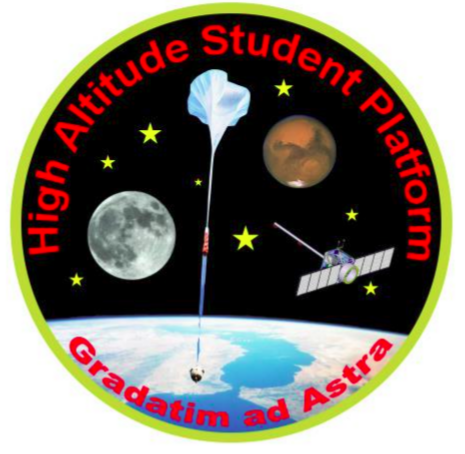
\includegraphics[width=0.08\linewidth]{Figures/logo.pdf}} %Header
\setlength\extrarowheight{4pt}

\makeatletter
\def\p@subsection{}
\makeatother
\makeatletter
\def\p@subsubsection{}
\makeatother

\fancyhf{}
\pagestyle{fancy}
\headheight 50pt
\lhead{\hasplogo} %Header
\chead{\vspace*{-2cm}\Large\textbf{HASP Payload Application 2019}} %Header
\rfoot{\thepage}

\parskip = 6pt %changes spacing between paragraphs


\begin{document}

\title{University of Houston HASP 2019 Application}

\begin{abstract}
  \begin{center}
    {\bf Abstract}
  \end{center}

  By learning from the methodology imposed by the previous SORA missions, the SORA 3 payload will feature improved systems to sample for extremophilic microorganisms and observe the stratospheric radiation environment.
  An overhauled system to capture microorganisms is being implemented by learning from what did and did not work on the previous SORA missions.
  Furthermore, the radiation system is expanding to include a container that will closely mimic an ISS module in terms of material structure in hopes of observing the radiation environment to which astronauts are exposed.
  In addition, the SORA 3 payload will implement a new system featuring organic photovoltaic cells in the interest of observing the change in performance and molecular structure of the cells as a result of prolonged exposure to intense radiation.
  The first two missions have established a technological foundation from which SORA 3 can expand through exploring more deeply the topics and challenges of the first missions. SORA 3 will continue to use hobby electronics to test the bounds of commerically available technology.
  
  \newpage %Breaks page for the Table of Contents.
\end{abstract}

\newcommand{\Physics}{College of Natural Sciences and Mathematics, Department of Physics, University of Houston, Houston, TX 77204, USA}
\newcommand{\CS}{College of Natural Sciences and Mathematics, Department of Computer Science, University of Houston, Houston, TX 77204, USA}
\newcommand{\Biology}{College of Natural Sciences and Mathematics, Department of Biology, University of Houston, Houston TX, 77204, USA}
\newcommand{\BME}{Cullen College of Engineering, Department of Biomedical Engineering, University of Houston, Houston TX, 77204, USA}
\newcommand{\Chemical}{Cullen College of Engineering, Department of Chemical and Biomolecular Engineering, University of Houston, Houston TX, 77204, USA}
\newcommand{\Electrical}{Cullen College of Engineering, Department of Electrical Engineering, University of Houston, Houston TX, 77204, USA}
\newcommand{\Mechanical}{Cullen College of Engineering, Department of Mechanical Engineering, University of Houston, Houston TX, 77204, USA}


%--- Add authors in the order they should appear
\author{R.~Masek}\affiliation{\Physics}
\author{J.~Patel}\affiliation{\Physics}
\author{M.~Butowicz}\affiliation{\CS}
\author{T.~Hill}\affiliation{\Physics}
\author{C. Amay}\affiliation{\CS}
\author{J. Arguello}\affiliation{\Mechanical}
\author{A. Boggs}\affiliation{\Physics}
\author{C. Bush}\affiliation{\BME}
\author{A. Elsaadi}\affiliation{\Mechanical}
\author{K. Fleming}\affiliation{\Chemical}
\author{S. Gupta}\affiliation{\Mechanical}
\author{D. Howard}\affiliation{\Electrical}
\author{E. Humble}\affiliation{\CS}
\author{A. Kalavadwala}\affiliation{\Mechanical}
\author{K. Ngo}\affiliation{\Physics}
\author{C. Rimbau}\affiliation{\Biology}
\author{J. Tristan}\affiliation{\Mechanical}
\author{H. Trong}\affiliation{\Mechanical}
\author{A. Vega}\affiliation{\Mechanical}
\author{S.~George}\affiliation{\Physics}
\author{I.~Wilson}\affiliation{\Biology}
\author{D.~Pattison}\affiliation{\Biology}
\author{P.~Gunaratne}\affiliation{\Biology}
\author{A.~L.~Renshaw}\affiliation{\Physics}



\setlength{\parindent}{1em}
\setdefaultleftmargin{1em}{1em}{}{}{}{}
\setcounter{page}{0}\thispagestyle{empty}
\maketitle
\onecolumngrid
\setcounter{tocdepth}{2}
\setcounter{page}{0}\thispagestyle{empty}
\tableofcontents
\setcounter{page}{0}\thispagestyle{empty}
\newpage

%---
%Section: Mission Overview w/ Subsections Mission Statement and Hypotheses
\section{Mission Statement and Objectives}
\label{sec:Introduction}


The 2019 University of Houston (UH) HASP team has set out to expand upon the previous missions \cite{SORA1}\cite{SORA2} from the UH team by applying the knowledge and technology that has accrued.
The methodology of the first two missions has provided a proof of concept for handling tools, such as the MiniPIX particle detector,  in extreme environments.
This will serve as the platform for the 2019 mission.

The main objectives of the 2019 mission is to study the exposure to ionizing radiation that organisms face in the upper atmosphere and sample these organisms and bring them to the surface.
The organisms in question are microbial extremophiles that naturally reside in this region of the atmosphere. 
However, we are also interested in the humans that reside in such harsh environments.
We will construct a thermally-controlled, pressurized mock-up International Space Station (ISS) module containing a scintillated MiniPIX.
The pressure will be held constant at \SI{1}{atm} to replicate conditions aboard the ISS.
This allows us to study the particle cascades induced by the materials of the module, which will give information regarding the dose that astronauts are exposed to while in space.
The payload will also contain a second, unscintillated MiniPIX that will reside outside of the ISS module, recording the outside radiation exposure.
This second MiniPIX will act as a control for the ISS module, but also allows us to study the environment that extremophiles are exposed to.
In addition to the MiniPIX, we will test the performance of organic photovoltaic cells in stratospheric conditions.
Organic photovoltaic cells have promising applications for space-based missions due to their inexpensive, lightweight, and durable nature relative to their non-organic counterparts.
In tandem to the radiation study, we will collect samples of the microbial life through the use of a passive collection system.
This system will consist of a T-shaped arm covered with filters that will only be exposed to the outside while at float altitude.
We will then bring the uncontaminated, collected samples down to the surface for analysis.

\noindent The upcoming mission has the following scientific objectives:

\noindent \textbf {Primary Scientific Objectives:}
\begin{enumerate}
\item Capture microorganisms in the upper atmosphere at altitudes of approximately \SIrange{30}{41}{\kilo\meter} using a method not previously used by the UH HASP team. 
\item Study the cosmic and terrestrial radiation that extremophiles and astronauts are exposed to.
\item Observe the influence of intense radiation on the structure and performance of organic photovoltaic cells.
\end{enumerate}

\noindent \textbf {Secondary Scientific Objectives:}
\begin{enumerate}
\item Testing the newly developed astrobiology hardware in flight and establish a more reliable method for collecting microbes in extreme environments at high-altitude.
\item Implement a redundant storage system for all data recorded.
\item Establish a methodology which allows two or more MiniPIX devices to be used in conjunction.
\item Study and test the performance of organic photovoltaic solar cells in the intense radiation environment.
\end{enumerate}

\noindent \textbf {Engineering Objectives:}
\begin{enumerate}
\item Develop a new astrobiology collection mechanism that is favorable at high altitude.
\item Construct a structure resembling an ISS module as accurately as possible.
\item Use a scintillator to detect thermal neutrons using a MiniPIX.
\item Analyze MiniPIX data in real time and downlink relevant information.
%\item Test an improved enclosure against impacts and harsh environments.
\end{enumerate}


\subsection{Hypothesis and Objectives}
\label{subsec:Hypothesis-Objectives}
\begin{enumerate}
\item By comparing our flight sample to previous missions \cite{SORA1}\cite{SORA2}, the newly developed passive astrobiology system can be quantitively and qualitatively be compated to previous methods.
  \begin{enumerate}
  \item Objective: Sample a comparatively larger volume of air using passive design elements rather than an active pump design at float altitude.
  \item Objective: Compare the effectiveness in rotation of the sampling filters to those that are stationary.
  \end{enumerate}
\item Background sampling and rigorous sterilization procedures will help rule out contamination as a possible source of error.
  \begin{enumerate}
  \item Minimize outside contamination of the entire astrobiology system.
  \item Objective: Retain a sterile environment for the entirety of the balloon flight.
  \item Objective: Sample a minimum volumetric amount of air at target altitude for the duration of the float phase (approximately 15 to 18 hours).
  \item Objective: Take background samples using Fluropore Membrane filters at the various locations where the payload will be.
  \end{enumerate}
\item The radiation environment within the ISS module will be noticeably different than that outside the module in terms of particle type and concentration. 
  \begin{enumerate}
  \item Objective: Characterize the radiation environment within the ISS module by particle types and dose.
  \item Objective: Successfully identify neutron interaction with the scintillated MiniPIX.
  \item Objective: After capturing samples, analyze data and compare biological effects to similar genotypes found on Earth's surface.
  \end{enumerate}
\item The organic photovoltaic cells exposed to stratospheric conditions will under perform cells which have remained on Earth.
  \begin{enumerate}
  \item Objective: Compare quantitative and qualitative properties of the cells such as fill factor, efficiency, and physical structure of post-flight cells to cells that have remained on Earth.
  \item Objective: Using microscopy techniques, analyze the influence of stratospheric radiation on the structure of the cells.
  \end{enumerate}
\end{enumerate}
  
\vspace*{-0.5cm}
\section{Background}
    \subsection{Astrobiology}
\label{sec:AstrobiologyBackground}

Extremophiles thrive in physically and/or chemically extreme conditions, which are detrimental to most of life on Earth as we know it. These organisms and microbes have been found everywhere, from deep underwater volcano vents to buried ice lakes in Antarctica \cite{Extremophiles}.  As shown in Table~\ref{tab:AstrobiologyTable}, fungi and bacterial spores have previously been found in the stratosphere. Arguably, each successful collection expedition of at least \SI{30}{\kilo\meter} into the upper atmosphere provides information that could be useful in determining what life forms can exist inside and outside of Earth's biosphere. Today, the most common altitude for bacterial collection in the atmosphere occurs in the range of approximately \SIrange{10}{20}{\kilo\meter} above Earth's surface; very little data exists on microbiological samples captured in the stratosphere. Conditions at altitudes of \SIrange{30}{40}{\kilo\meter} are extreme in temperature, pressure and radiation. 
	
%\begin{figure}[H]
%\centering
%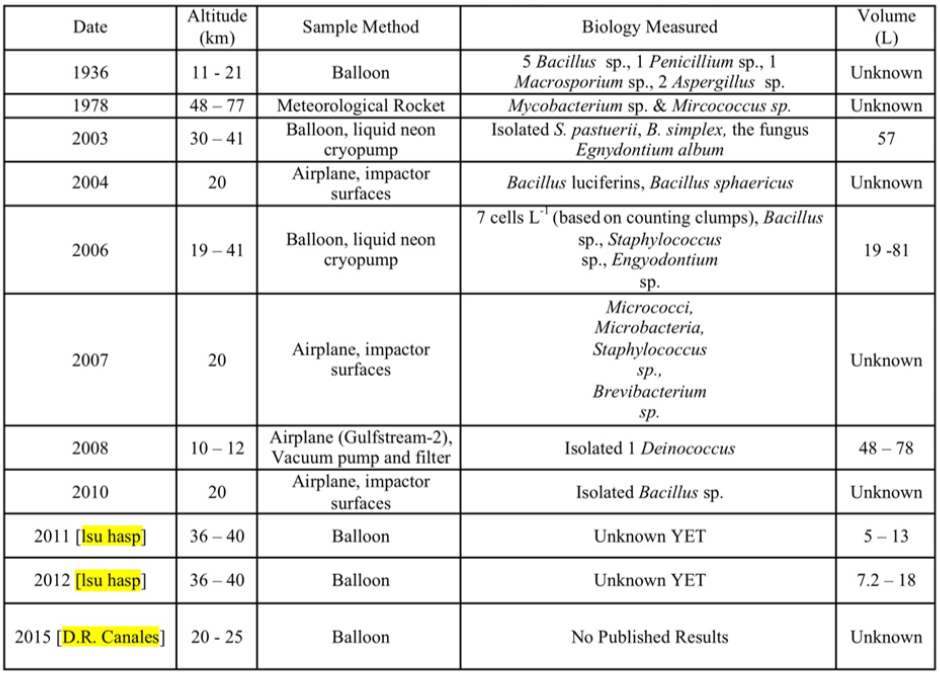
\includegraphics[width=1\textwidth]{./Figures/AstroChart.PNG}
%\caption{}
%\label{fig:AstroHist}
%\end{figure} 

Our experiment is an attempt to further develop our technique for capturing microorganisms in the upper atmosphere, as demonstrated during our 2017~\cite{SORA1} flight; which was inspired by the LSU HASP 2011, 2012, 2013 flights~\cite{LSU} and from research by D.R. Canales~\cite{Canales}.  This flight will help confirm the results from our first flight and potentially enable us to culture these rare microorganisms.  We will use two of the KNF N84-4 commercial gas-sampling diaphragm vacuum pumps to sample the air at approximately \SI{33}{\kilo\meter} above Earth's surface. The samples we hope to collect are an important part to expanding our understanding of Earth's biosphere. Further studies could provide more insight on how life can be distributed on Earth, and ultimately, through outer-space.

\begin{table}[!ht]
  \centering
  \caption{History of Microbiological Sampling of the stratosphere~\cite{SORA1}.} 
  \bigskip
  \begin{tabular}{c c c p{6cm} c}
    \hline
    \hline
    \multicolumn{1}{c}{\bfseries Date} & \minitab{c}{\bf Altitude}{\bf (km)} &  \multicolumn{1}{c}{\bfseries Sample Method} & \multicolumn{1}{p{6cm}}{\bfseries Biology Measured} & \multicolumn{1}{c}{\bfseries Volume} \\
    \hline
    1936 & 11 - 12 & Balloon			 		& \minitab{l}{5 Bacillus sp., 1 Penicillium sp.,}{1 Macrosporium sp., 2 Aspergillus sp.} 	  & $Unknown$ \\ \hline
    1978 & 48 - 77 & Meteorological rocket 		        & \minitab{l}{}\par Mycobacterium sp., Mircococcus sp.					          & $Unknown$ \\ \hline
    2003 & 30 - 41 & Balloon, liquid neon cryopump	        & \minitab{l}{Isolated S. pastuerii, B. simplex,}{the fungus, Egnydontium album}       		  & $57$      \\ \hline
    2004 & 20	   & Airplane, impactor surfaces 	        & \minitab{l}{}\par Bacillus luciferins, Bacillus sphaericus			                  & $Unknown$ \\ \hline
    2006 & 19 - 41 & Balloon, liquid neon cryopump              & \minitab{l}{7 cells L-1 (counting clumps), Bacillus sp.,}{Staphylococcus sp., Engyodontium sp.} & $19-81$   \\ \hline
    2007 & 20	   & Airplane, impactor surfaces 	        & \minitab{l}{Micrococci, Microbacteria,}{Staphylococcus sp., Brevibacterium sp.}    		  & $Unknown$ \\ \hline
    2010 & 20	   & Airplane, impactor surfaces                & \minitab{l}{}\par Isolated Bacillus sp.							  & $Unknown$ \\ \hline
    2017 & 32	   & Balloon, liquid medium w/ vacuum pump	& \minitab{l}{}\par Multiple findings~\cite{SORA1}					          & $Unknown$ \\ \hline
    2018 & 32	   & Balloon, liquid medium w/ vacuum pump	& \minitab{l}{}\par Inconclusive~\cite{SORA2}							  & $Unknown$ \\ \hline
  \end{tabular}
  \label{tab:AstrobiologyTable}
  \medskip
\end{table}

    \subsection{Cosmic Radiation}
\label{subsec:RadiationBackground}

Understanding the biological effect of radiation on humans is cruicial for successful space flight.
By observing the environment in which astronauts reside, information regarding the conditions which induce the biological changes can be gathered.
Among this information is dosage of various particles.
In the upper atmosphere, primary particles, which consist largely of protons (p\textsuperscript{+}) and ionized atomic nuclei \cite{Frank}, collide with the nuclei of air molecules and can induce air showers.
These air showers produce secondary particles, which consist of positrons/electrons (e\textsuperscript{$\pm$}), neutrons(n), muons($\mu$\textsuperscript{$\pm$}), pions ($\pi$\textsuperscript{$\pm$}), and various other hadrons.
The primary particles of interest are Galactic Cosmic Rays (GCRs), which originate outside of the solar system but within the Milky Way Galaxy and typically have been accelerated to nearly the speed of light \cite{GCRs}.

The results from the previous missions have confirmed the successful application of the MiniPIX as a dosimeter through the idenification of the Regener-Pfotzer Maximum. This maximum is the altitude at which ionizing radiation reaches its peak \cite{Regener}. The value of this altitude depends on various environmental factors, but it is around \SI{18}{\kilo\meter}. With this confirmation, the MiniPIX will remain the primary tool we will use to measure radiation.

Primary particles can induce an air shower by colliding with the nucleus of any atom or particle.
This poses a potential threat to astronauts residing in spacecrafts, as the materials in the spacecraft's structure can induce an air shower and thus bombard astronauts with radiation.
By using a MiniPIX to measure the radiation outside of as well as within a structure emulating a module from the Internation Space Station, we can observe the environment that current astronauts live in and how the structure changes the radiation field.
Additionaly, the measurements outside of the structure will give information as to the conditions in which atmospheric extremophiles reside.

\subsection{Organic Solar Cells}
\subsubsection{Introduction}
Photovoltaic devices have been a staple in space energy harvesting since the launch of Vangaurd 1 in 1958. Since then, silicon, gallium arsenide, indium phosphide, cadmium telluride, and other III-IV systems have played the key roles. When choosing a system to gather solar energy, the only economic factors are the initial cost of the arrays, and the cost of transporting the system to orbit. To reduce this cost, we want solar cells with the highest specific power, which is defined as the W/kg. Recent studies have shown organic solar cells (OSC) with a specific powers of 10 W/g, which is why OSCs are an active area of research for space energy generation. Organic solar cells are thin film, light weight, flexible, and can be produced using roll to roll printing, making it ideal for space applications. In this experiment, we are exploring the effects of stratospheric conditions on organic solar cells, with a particular focus on the effects of cosmic ray bombardment in conjunction with the MiniPIX system, as well as to investigate the radiation hardness of different types of organic solar cells and demonstrate their reliability upon entry and exit of the stratosphere. In the following sections we will explain the basic workings of an OSC and explain some of the benifits and hinderences of a space like environment on the OSC, then explain the methodology of our experiment.\cite{Space organic cells}

\subsubsection{Working principals}
OSCs use earth abundant, carbon based semiconductors, such as conjugated polymers(as donors) and fullerene derivatives(as acceptors). Where as in mono-crystalline solar cells the valance and conduction bands are used to determine the energy band gap, OSCs model the difference between the highest occupied molecular orbit(HOMO) and the lowest unoccupied molecular orbit(LUMO) as equivalent to this energy band gap. When donor(D) and acceptor(A) layers meet, their Fermi levels match up and band bending occurs, which creates a small electric field, or built in potential (Vbi). Charge generation occurs when excitons, an electron/hole pair bound together by the Coulomb force, are generated in the donor material. This exciton will travel towards to D-A interface, where the aforementioned Vbi will seperate the exciton into free charges given sufficient conditions.  Exciton transportation inside of the bulk is hindered to 5-50nm before recombination occurs depending on material and structure, while the average thickness of an OSC is 50-100nm, thus the architecture of the active layer is of much importance. Instead of using a bi-layer of n-type and p-type semiconductors, OSCs use the bulk hetero-junction (BHJ), which is a blend with A-D regions that are within the estimated diffusion length.  
	
A newer type of organic-inorganic blend solar cell which has gained a lot  attention is the perovskite solar cell (PSC). This solar cell has a novel active layer comprised of organometallic molecules which exhibit the perovskite crystal structure ABX3. The most commonly used perovskite material is methylamoniumm lead trihalide (CH3NH3PbX3, MAPX), where lead can be swapped for tin, and halides such as boron, iodine, and chlorine are employed. Fabrication of the perovskite solar cell is highly attractive as it can be accomplished with wet chemistry, roll to roll printing, or vapor deposition. Some key features of the perovskite structure is that the bandgap of the material is tunable via the halide content and that the diffusion length of holes and electrons is ~1 micron, making them perfect for roll to roll thin film printing. The Shockley–Queisser limit is about 31 percent under an AM1.5G solar spectrum at 1000W/m2, for a Perovskite bandgap of 1.55 eV, which is near the theoretical maximum of 33.7 percent, and reports of perovskite cells with PCE as high as 22 percent have already been fabricated. As a newer material there is still much unknown about the physics of the perovskite solar cell, such as if charges occur as bound excitons or free charges.

Space transport involves high doses of radiation, large fluctuations of temperatures, and extreme vacuum conditions. The need to study the effects of a space like environment on organic electronic devices is paramount as advances in the organic semiconductor field continue and space exploration becomes more standard. In this study, we propose to mount four different types of solar cells onto our payload and monitor their performance. We will be using prefabricated small molecule based OSCs, self fabricated polymer based OSCs, self fabricated PSCs, and prefabricated amorphous silicon solar cells. Each of these is a lightweight, flexible, and thin solar cell ideal for space use. Additionaly, effect to the crystal structure of the perovskite based cell is of particular interest, as cosmic ray bombardments and fluxtuations of temperature can be determental. 
	


%\subsubsection{Solar Radiation}
%The ultraviolet (UV) spectrum is composed of UVC (\SIrange{200}{280}{\nano\meter}) with only \SI{0.5}{\percent} of the entire solar spectrum, 1.5\% of
%UVB (\SIrange{280}{315}{\nano\meter}) and UVA (\SIrange{315}{400}{\nano\meter}), which contributes to \SI{6.3}{\percent}~\cite{uv_irradiance}. UVB and UVC are the main contributors in highly lethal solar radiation to microorganisms\cite{UVonDNA}. DNA is prone to high absorption levels at those wavelengths, often causing inactivation and mutation.  Therefore, understanding the exposure of microbes in to UV radiation is quite important.

%In the atmosphere ionizing radiation does not always increase with altitude. As
%primary GCRs such as high energy protons, alpha particles, and 
%heavy ions collide with atoms in the atmosphere they begin to shatter into secondary
%particles such as neutrons, pions, electrons and muons which causes a peak in 
%ionizing radiation at around \SI{18}{\kilo\meter}. This peak is known 
%as the Regener-Pfotzer Maximum\cite{regener} and shows that with increasing atmospheric density
% ionizing radiation increases until peaking high in the stratosphere and then decreases rapidly as you 
%reach the surface of the earth.



%Expand upon Regener-Pfotzer Maximum. Refer to other papers to validate the range. 
%The intensity of GCR peaks within a range of about
%\SI{18}{\kilo\meter} to about \SI{22}{\kilo\meter} []. This range,where the production of ionizing radiation reaches its
%peak is known as the Regener-Pfotzer Maximum\cite{regener} . The Regener-Pfotzer Maxiumum is unique and is dependent on
%location and time of the year, as it is determined by a number of
%factors, which include but are not limited to the strength of earth's
%electromagnetic field, atmospheric composition (specifically ozone
%content(?){\bf The intensity of the cosmic ray flux and the secondary
%  environment vary inversely with the solar cycle due to the
%  interaction of the earths electromagnetic field. In addition, the
%  sporadic solar events that occur in short busts can increase the
%  primary particle flux periodically (hours to days) can in fact
%  enhance the atmospheric radiation several orders of magnitude in
%  scale.}), the sun's relative position, and maximum solar elevation
%[]. The combination of these affects results in a variability in the
%location of the maximum as well as the existene of this maximum as
%ooposed to an ever-increasing intensity.



%Payload Design and Operation
\section{Payload Systems and Operation}
\label{sec:PayloadSystems}
    \label{sec:Hardware}

SORA 3 will implement an overhauled astrobiology system that will collect larger samples of stratospheric organisms as well as require less amperage, allowing us to expand the radiation system and reduce the chance of electrical failure. The radiation system will apply the techniques developed over the previous missions by consisting of a scintillated MiniPIX within a pressurized module modelled after an ISS module. Additionally, various types of organic photovolatic cells will be flown in order to study their performance in harsh stratospheric conditions.

    \subsection{Astrobiology System}
\label{sec:AstrobiologySystem}

\subsubsection{Design and Operation}
The collection assembly will be designed as a one mechanized enclosure as shown below. The rotating arm will be raised out of the collection container and began rotating once float altitude has been reached. The raising of the rotating arms will be done by a L-16 linear servo motor. The rotation of the filter arm will be provided by the rotational motor mounted onto the filter arm. The lid on the top of the linear servo will seal the clean box during ascent and descent. The  Fluropore Membrane filters will be mounted on the ends of the rotating arm. The arms will spin at 80 RPM for the duration of float conditions. In theory, the sampled volume will be the cross-sectional area of each filter multiplied by the distance the payload travels, which results in a far greater sampled volume than the 0.03 liters per minute sampling of the pumps from the previous flight.\cite{SORA2} When it is time for the payload to descend, a command will be sent to retract the rotating mechanism back into the clean box. The fluropore filters on the rotation arm will be compared to the ones on mounted on the linear servo as shown in the figure below. Background samples will be taken using the same fluropore membrane filters and will sample the various places the payload will be, such as the UH lab room, the clean room used for sterilization and the Fort Sumner launch site. 

\begin{figure}[!h] 
	\begin{center}
		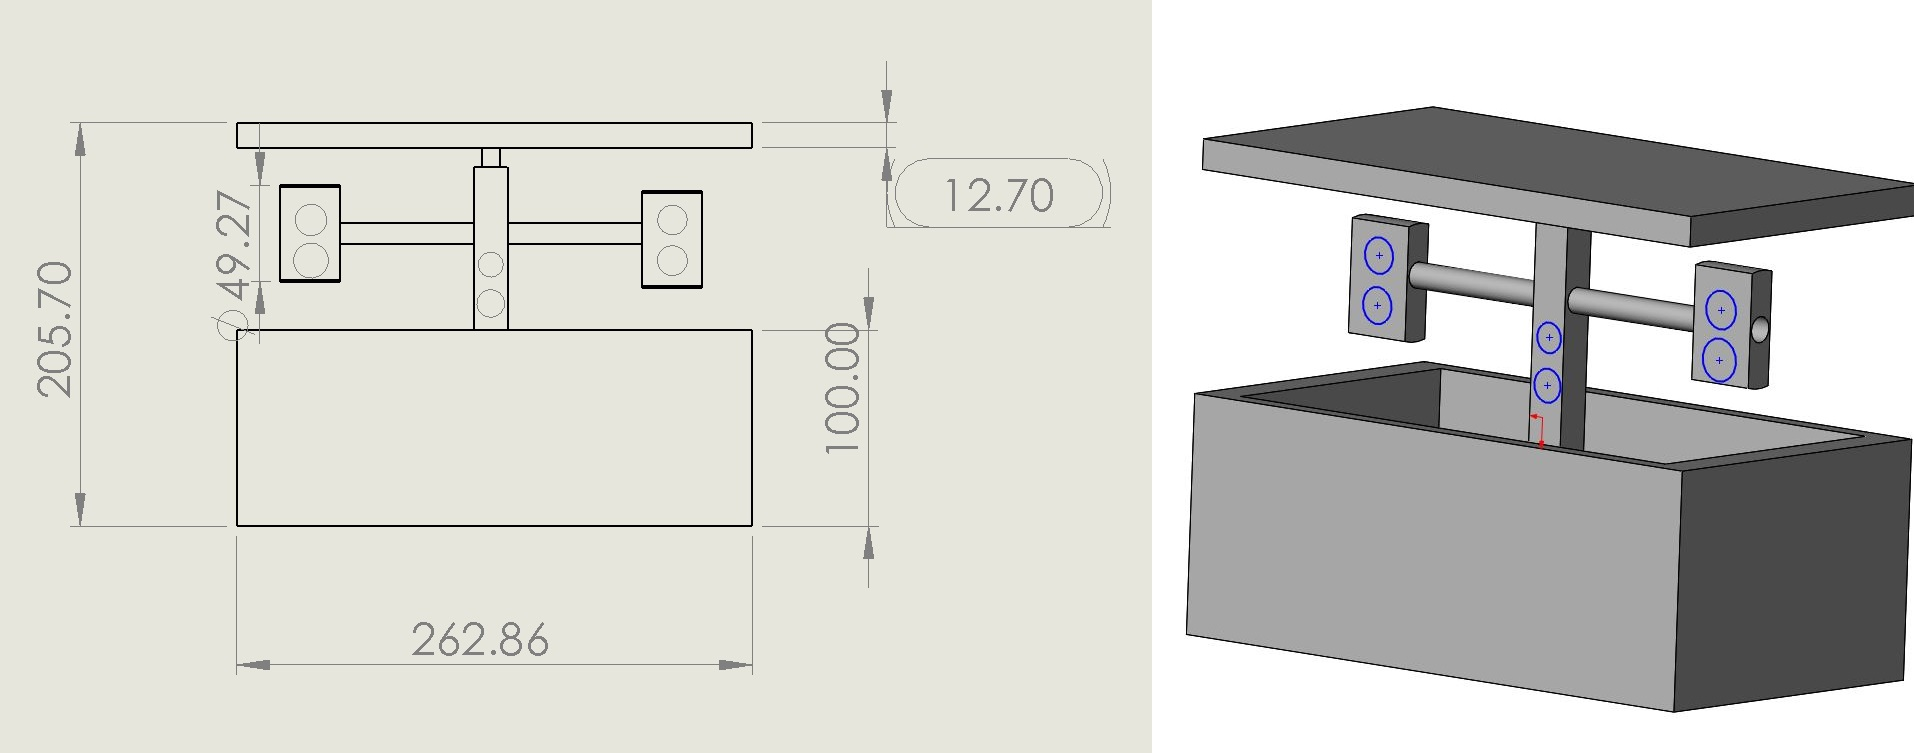
\includegraphics[width=\linewidth]{Figures/T-Arm.jpg}
		\caption{Cross-section view of the clean box with the extended rotating arm. \bf All numbers are in millimeters}
		\label{fig:AstroBox}
	\end{center}
\end{figure} 
%\subsection{Astrobiology Methods}
%\label{sec:Astrobiology Methods}
\subsubsection{Pre-Flight Preparation}
The rotating arm mechanism will be tested in low pressure and in various mounting positions. Once it is certain that the arm functions in the intended conditions during flight. We will take it to the clean room to be sterilized.  

The clean box that houses the arm  will autoclaved. All tools used in the assembly of the clean box will either be autoclaved or soaked in a \SI{70}{\percent} ethanol solution inside of a clean room. Each person who enters the clean room will be garbed in a lab coat, goggles, hair net and latex gloves after thoroughly washing their hands in a \SI{70}{\percent} ethanol solution.All wires within in the box will be soaked in the \SI{70}{\percent} ethanol solution and the rotating arm mechanics will be powered on and retracted the box. The box will then be integrated into the payload. 
\subsubsection{Post-Flight Procedures}

Once the payload is retrieved, the intact clean box needs to be removed and placed inside of a cooler with ice to be then transported to The University of Houston and placed in cold storage at \SI{4}{\celsius}. All equipment used in the filtration process will be either autoclaved or taken from previously unopened sanitized packaging. The autoclaved, pre-sanitized items and the clean box will then be washed in a \SI{70}{\percent} ethanol solution before they are placed inside a SterilGARD e3 Class II Biological Safety Cabinet (the Cabinet). The cabinet has a laminar flow air barrier and UV lights built into the ceiling for decontaminating the workspace prior to use.The Fluropore Membrane filters from the clean box and the backgeound samples will be processed through a DNA extraction kit and the remaining sample fluid will be stored in the cold storage for in-house 16S ribosomal RNA sequencing through the University of Houston sequencing team.  


    \subsection{Radiation Monitoring System}
\label{sec:RadiationDesign}

\subsubsection{MiniPIX Detector}
The MiniPIX detector is a silicon-based hyrbid pixel detector founded on Timepix technology. The device is built by ADVACAM \cite{Advacam}  and utilizes technology developed by the Medipix Collaboration at CERN \cite{Medipix}. The sensor consists of a \num{256}x\num{256} array of pixels and a pitch of \SI{55}{\micro\meter}. A USB 2.0 connection is used to interface with the device, which provides power and data output. The primary use of the detector will be to characterize cosmic radiation by the type of particle and its incident energy.
%The device is capable of operating in the following three different modes: single particle counting, Time-over-Threshold, and Time-of-Arrival.

\begin{figure}[H]
  \begin{minipage}[c]{0.40\linewidth}
    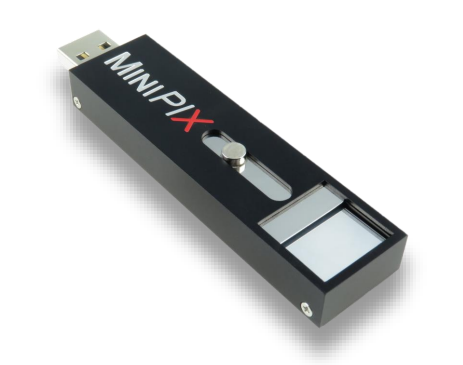
\includegraphics[width=\linewidth]{Figures/Minipix2.png}
    \caption{Picture of a MiniPIX particle detector~\cite{Advacam}.}
    \label{fig:Minipix}
  \end{minipage}
  \hfill
  \begin{minipage}[c]{0.45\linewidth}
    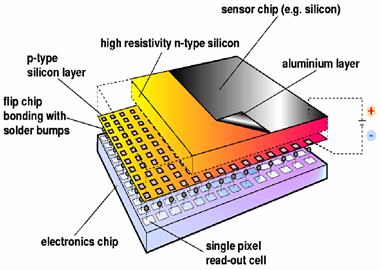
\includegraphics[width=\linewidth]{Figures/MinipixLayers.png}
    \caption{Layers that makeup the MiniPIX sensor.}
    \label{fig:MinipixLayers}
  \end{minipage}
\end{figure}

When an ionizing particle hits the sensor, electron-hole pairs accumulate within the semiconducting material. The electronics reads-out the pairs by depleting the silicon with a bias voltage. If a charge is above the set threshold, the charge is counted. The energy deposited in a pixel can be determined from the back-plane pulse amplitude. Particles incident on the sensor appear as pixel clusters, which is defined as a continuous area of activated pixels. By analyzing these clusters, the incident particle can be identified. The morphology of the cluster gives information regarding the type of particle as well as the angle at which the particle was incident upon the detector. 

Detectors using Timepix technology are used to measure radiation aboard the ISS. Since the University of Houston is a member of the Medipix Collaboration, scientists at the University of Houston work with preparing Medpix devices to be used aboard the ISS. As a result, the UH HASP team may be able to work with these scientists and compare data gathered from the mockup ISS module to data from the ISS.

Due to the SORA 3 mission being a continuation of previous missions, we have the opportunity to compare data from previous flights. For example, this will allow us to observe how data regarding particle counts and dose changes with the solar cycle. Hathaway \cite{Hathaway} has shown that a direct relationship exists between the development of the solar cycle and neutron counts.

\begin{figure}[h]
    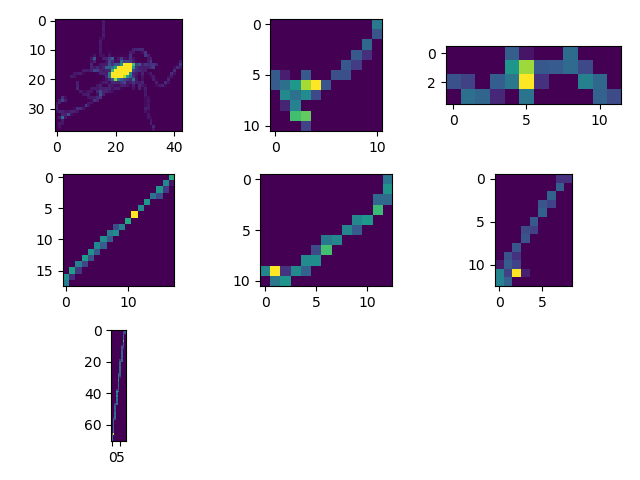
\includegraphics[scale=1, width=.75\textwidth]{Figures/Tracks.png}
    \caption{Examples of different track types from data collected by a MiniPIX.}
    \label{fig:Tracks}
\end{figure}

\subsubsection{Calibration}   
It is necessary to calibrate the sensor. The calibration procedure is rather sophisticated, so the calibration will be applied by Dr. Stuart P. George at the University of Houston. Dr. George is a member of the Medipix Collaboration. The general outline of the calibration is as follows. A source calibration is applied by using a \SI{60}{\keV}{\ce{^241Am} decary line, \ce{Sn} Flourescence and \ce{^55Fe} gamma rays. The pixel detector consists of \num{65536} silicon p-n dioded, each containing its own individual processing circuit. The response of each pixel can never to identical to one another, so a calibration mut be performed on each pixel. Dr. George will calibrate each pixel energy threshold from DAC counts to energy \cite{StuartThesis}. The threshold of the sensor will be set to \SI{4}{\keV}, which sufficiently filters out background noise. The bias voltage of the sensor will be set to \SI{200}{\volt}, which guarantees that the silicon is completely depleted while reading out the charge.
  
\subsubsection{Collection Parameters}
% Put the settings for the minipix shutter time, bias voltage etc. here
ADVACAM has developed a Python API to configure the device and its acquisition parameters. The shutter speed of the device controls the rate at which data is output from the device. The shutter speed controls the exposure time of the sensor before saving the data to a frame. Once the data is saved, the device enters manufacturer-set dormant period, which lasts for approximately two seconds. This time will be utilized as a cool-down period for the device. The value of the shutter speed is highly dependent on the application of the sensor. Within the context of HASP, we expect high radiation exposure which will require a quicker shutter speed. This is to the fact that if the shutter speed is too long, the sensor become overcrowded and clusters become difficult or impossible to analyze. However, if the shutter speed is too short, there will be many frames with little to no data, which will use a large amount of storage space. Based off of previous SORA missions, a shutter speed of a few seconds is sufficient for our application. The exact shutter speed will be determined through testing and may be different for each device we use.

\subsubsection{Data Format}
The data frames are stored as plain text values where each value corresponds to a value from a pixel on the pixel array. In a separate file, metadata such as acquisition type, shutter speed, bias voltage, and other parameters are recorded for each frame. Both the data file and the metadata file will be stored on the RP\num{3} and the various redundant storage systems we implement. The MiniPIX data from previous missions used about \SIrange{1}{2}{\giga\byte}. For the 2019 mission, we expect about double that value due to our use of two MiniPIX devices.

\subsubsection{Structure}
The MiniPIX outside of the ISS module will be contained within a small case plastic case to protect the device from atmospheric moisture. Thermal paste will be used to fix the MiniPIX on a small block of aluminum, which will behave as a heat sink. This simple setup has proven to work on previous missions and is shown in Figure \ref{fig:CaseAssembly}.
\begin{figure}[h]
    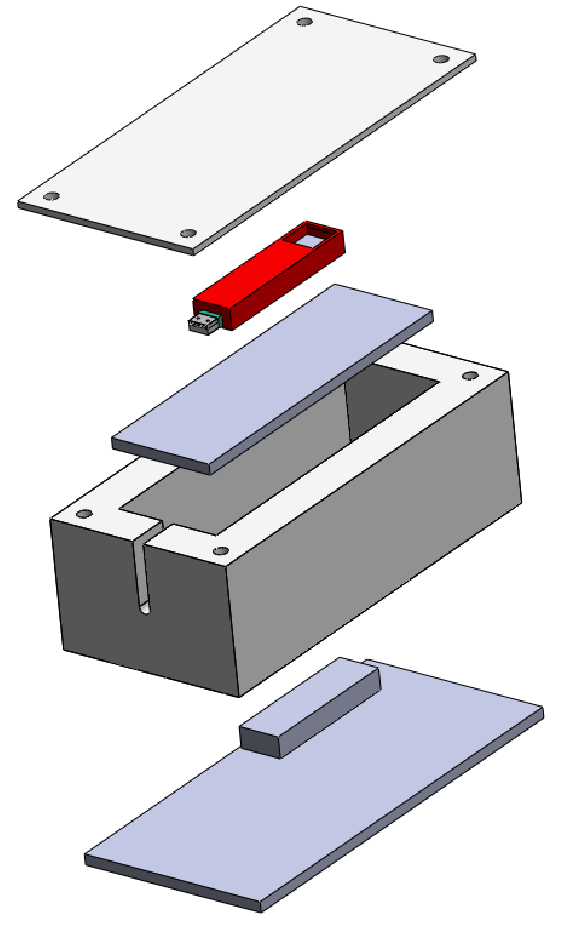
\includegraphics[scale=1, width=.25\textwidth]{Figures/MinipixCaseAssembly.pdf}
    \caption{Exploded view of the MiniPIX case assembly. Shown in white is the plastic construction, red is the MiniPIX device, and the grey represents the aluminum heatsink.}
    \label{fig:CaseAssembly}
\end{figure}

\subsubsection{ISS Module}
\label{subsec:ISSModule}
As part of the radiation subsystem, the payload will include a capsule intended to mimic the structure of one of NASA's modules on the ISS.
The method deployed by NASA and other agencies is called ``Stuffed Whipple'' shielding and is deployed in ISS modules that are at highest risk of impact \cite{NASAShielding}.
This module will remain at atmospheric pressure throughout the entire flight in attempt to model the environment as closely as possible.
Inside the capsule will be a scintillated MiniPIX that will record the radiation environment within the module.
The scintillated MiniPIX will measure the neutrons within the ISS structure in attempt to determine the exposure within the structure.

The materials that make-up the module will be those used in the outer walls on the ISS and will have the same thickness.
The main differences in structure will be the omission of standoffs and a multi-layer insulator (MLI) in our module.
The walls of the ISS have standoffs between layers of materials, which increases the total wall thickness to about one foot, and the MLI used by NASA is not available commercially.
%Due to being in space, the gaps between the layers are a vacuum.
In the interest of saving space, we will not include the standoffs, and all materials will be layered on one another in the same order as they are used on the ISS.

\begin{figure}[H]
  \centering
  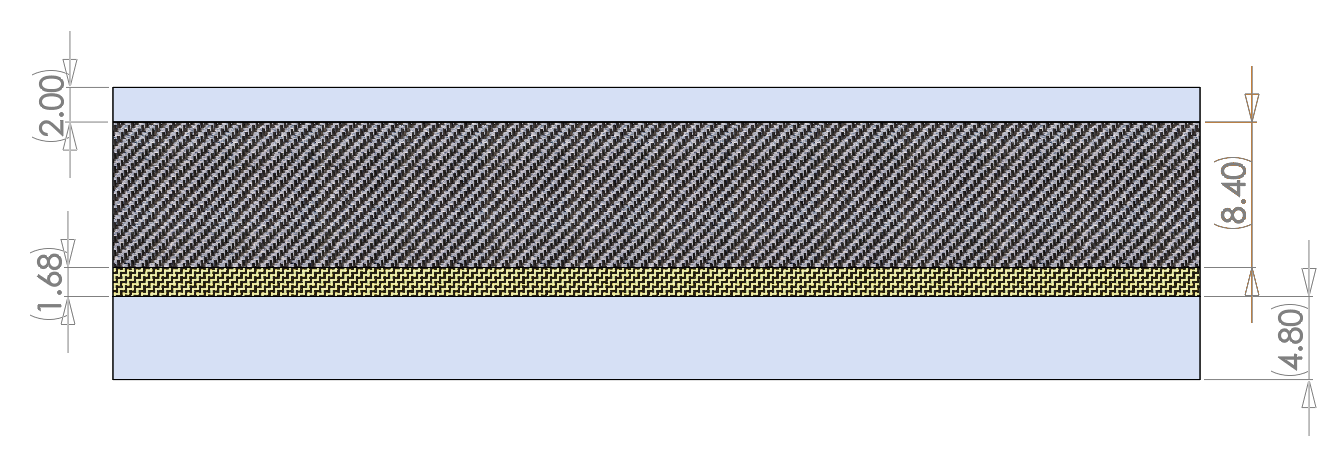
\includegraphics[width=0.8\linewidth]{Figures/MaterialCrossSection.png}
  \caption{Layers and thicknesses of the materials that will be used to construct the ISS module. From top to bottom: aluminum 6061-T6, six layers of Nextel AF62, six layers of Kevlar fabric, and aluminum 2219-T87. The atmosphere is contained by the \SI{4.8}{\milli\meter} layer of aluminum \cite{NASAPP}. All measurements are in \si{\milli\meter}.} 
  \label{fig:ISSLayers}
\end{figure}

%To construct the module, a rectangular box of aluminum will be constructed with one missing face, constituting the inner aluminum box that will contain the pressurized environment. The 

\subsubsection{Scintillated MiniPIX}
The MiniPIX's sensor can only interact with charged particles. In order to measure neutrons with the MiniPIX, a scintillator is rerquired. The scintillator will interact with the neutrons and produce a specific signature of particles which can be measured by the MiniPIX. Uher et al. \cite{Uher} used a similar method, but with a lithium-based scintillator. We will use a boron-loaded plastic scintillator \cite{BoronScintillator} to cover exactly half of the MiniPIX sensor. The reation between the Boron-10 nucleus and a thermal neutron is \[\ce{^10B + n -> ^7Li + ^4He + \gamma (\SI{480}{\kilo\eV})}\] according to Pawelczak et al \cite{Pawelczak}. This scintillator was chosen due to its large reaction cross-section for thermal neutron capture and its emission of light charged particles. This larger rwaction cross-section increases the probability that the neutron will produce particles that can be measured by the MiniPIX.

By covering half of the sensor, we can compare the uncovered half with the data recorded by the MiniPIX outside of the ISS module.

\subsubsection{Organic Photovoltaic Cells}    
We will be using four different types of solar cells with a total of 12 arrays on board our payload. There will be one type of cell on each of three sides of the payload, leaving one face free for any unique cells we may develop during our research. Half of our panels will be prefabricated and purcahsed from a supplier, and will be regarded as a control against which we will evaluate our in house fabricated cells. For the in house fabrication, we will be focusing on polymer:fullerne BHJ and perovskite active layer cells. We intend to investigate a variety of polymer:fullerene blends and develop a procedue for fabrication which yields the greatest PCE and MPP in the stratospheric environment, and to investigate the possibility of transpatent conductive oxide(TCO) layers besides the traditional indium tin oxide (ITO) glass and polyethylene terephthalate (PET) plastic. 

Solar cells are characterized by their current vs voltage (IV) curve, which tells you the maximum power point ($MPP$), $V_{max}$ and $I_{max}$, open-circuit voltage ($V_{oc}$ and short circuit current ($I_{sc}$), leading to the fill factor ($FF$) and efficiency ($PCE$). This curve will be  generated using a variable resistor in series with two multimeters, one acting as voltmeter and the other an ammeter, and the solar cell in question, which will follow Ohm's Law. From the plot, $V_{oc}$ is seen when $I=0$, $I_{sc}$ is when $V = 0$, and the $MPP$ is where $V_{max}$ and $I_{max}$ meet. The $MPP$ can then tell us the efficiency ($Eff$), which is defined as
\begin{equation}
  Eff = \dfrac{MPP}{P_{in}}.
\end{equation}
The fill factor gives information on the "squareness" of the IV curve and is defined as
\begin{equation}
  FF = \dfrac{MPP}{V_{oc}I_{sc}},
\end{equation}
and it is optimal to maximize the fill factor. \cite{OPV operation}

Before flight, every cell will be characterized with IV curves using AMG 0 simulated sun light to generate a characteristic profile, as expected in the space environment, for the each new cell, and microscopy will be preformed to understand the topology and interfacial details of the new cells. Currently our plan is to have one of each cell type remaining on ground as a control, and we will have each panel onboard the payload wired to an arduino unit where IV curves will be recorded during flight, with a characteristic profile generated every \SI{30}{\second}. This data will be stored on the arduino with backup stored to a raspberry pi. On board our payload we will be measuring the tempreature and pressure of the environment to deteremaine any effects on the preformance due to temperature and pressure changes. Finally after recovery, the IV data will be extracted from the arduino/raspberry pi and plotted, and each cell will be re characterized and once again viewed under the microscope to look for any physical defects. 
    
With the HASP mission, we are going to compare fabricated organic polymer and perovskite solar cells against purchased prefabricated organic solar cells. Each of these cells will be analyzed before, during, and after exposure to the stratosphere. In analyzing our cells, we will measure the open circuit voltage, short circuit current, and maiximum power point, then fill factor will be determined along with efficieny.
In conjunction with our MiniPIX detector, we will be analyzing the effect that cosmic ray bombardment has on our solar cells. By analyzing the times at which cosmic rays are recorded, we can look at our IV data and determine if there was any effect on the cells preformance. Additionally, we will watch for problems which arise due to UV-A, B, and C rays with photodiodes. These photodiodes will serve the additional purpose of monitoring the solar power spectrum that our cells are exposed to.

    \subsection{SOCRATES Design}
\label{sec:ElectronicsDesign}

\subsubsection{Overview}

For this mission, we will use SOCRATES (System fOr Computing, Radiation, Astrobiology, Temperature, Environment and Solar), our flight computer, to manage flight operations and send and receive commands from the ground. SOCRATES is composed of two components: a Raspberry Pi 3 (RP3) and an Arduino Mega (Arduino) which interface via USB. SOCRATES' primary purposes during the flight will be to monitor environmental conditions inside the payload structure and inside the ISS module and to control the astrobiology system. It will also monitor temperature of the various subsystems including the solar cells, astrobiology collection system, MiniPIX, and air pressure throughout the flight. The temperature of each the 12 solar cells will be individually monitored with a thermistor. The voltage produced by each cell will also be monitored and recorded by SOCRATES via the Arduino. SOCRATES will use an accelerometer to monitor the activated state of the astrobiology system. All recorded data will be continuously written to an SD card mounted on a shield on top of the Arduino and to a removable USB flash drive connected to the RP3. SOCRATES will be programmed to deploy the astrobiology system at the appropriate altitude as sensed by the atmospheric pressure sensor. SOCRATES will also accept discrete commands from the HASP systems to turn the astrobiology collection system on and off.

In order to maintain data integrity we will save the data recorded by SOCRATES to both the SD card of the Arduino and to the USB drive connected to the Raspberry Pi. Data will be written to a discrete data file for a given period of time and then the file name will be incremented and the following data will be written to a new file. In case the data collection process is corrupted for a given period of time, this period of corruption will not interfere with the collection of all previous data. 

\subsubsection{The Sensors}

Our payload will utilize 14 thermistors to measure temperature at various points in our payload. The decision to use thermistors was based primarily on the performance of the analog temperature sensors during our 2017 flight, during which several of those sensors had slight malfunctions, and the success of thermistors in our 2018 flight. Thermistors are able to accurately measure temperature in the range \SIrange{-55}{125}{\celsius} and should therefore be adequate for the conditions in the stratosphere. Pressure will be recorded from two digital pressure sensors, one low pressure sensor in the main payload structure which will record pressure in the \SIrange{0}{3.44}{\kilo\pascal} range, and the second pressure sensor will be located inside the ISS module and record pressure in the \SIrange{20}{110}{\kilo\pascal} range. All sensor data will be UTC timestamped via the onboard real time clock and recorded to the SD card on the Arduino and USB drive attached to the RP3. To confirm the activated status of the astrobiology collection system, an accelerometer will be used to detect whether the collection arm is spinning or parked as is appropriate for the altitude of the payload. Each solar cell will also be monitored for temperature to aid in the calculation of efficiency of each cell. One MiniPIX will be located inside the ISS module and an additional MiniPIX will be located inside the main structure of the payload.

\begin{table}[h!]
\centering
\caption{Sensors that compose SOCRATES}
\label{tab:Sensors}
\bigskip
\begin{tabular}{cccc}
  \hline
  \hline
  \multicolumn{1}{c}{\bfseries Sensor} & {\bfseries Quantity} & {\bfseries Platform} & {\bfseries Purpose} \\
  \hline
  Thermistor          		& 4 & Arduino  		& Record temperature measurements  \\
  Pressure (\SIrange{0}{3.44}{\kilo\pascal})        				& 1 & Arduino 		& Record lower pressure measurements \\
  Pressure (\SIrange{20}{110}{\kilo\pascal})        				& 1 & Arduino 		& Record higher pressure measurements \\
  Accelerometer       		& 1 & RP3    		& Report the current state of astrobiology system \\
  Real Time Clock 				& 2 & Arduino/RP3 	& Record timestamps in UTC \\
  MiniPIX         				& 2 & RP3     		& Cosmic ray detector \\
  \hline
  \hline
\end{tabular}
\end{table}


\subsubsection{Space Constraints}
Since half of the space inside the payload will be used by the astrobiology systems, we need to design our electronics to be relatively compact yet accessible for necessary modifications or repairs after testing. We will use one RP3 to both interface with two MiniPIX and store sensor and voltage data from the Arduino.  Also, in order to reduce the space required for the interface between the Arduino and all of the payload's sensors, we will use two layers of proto-shields to more effectively utilize vertical space. The RTC pressure sensors will be mounted directly on the first shield while the thermistors will be mounted on the top most shield. 

\subsubsection{Powering It Up}
 In order to stay within the power constraints, a robust power supply will need to  handle all the components of the payload.  The power supply we will be using is the PCM-DC-AT500 by WinSystems INC.  It offers one \SI{+5}{\volt} needed to power the payload's electronics.  This power supply could effectively take \SI{+30}{\volt} and step it up to the \SI{+12}{\volt} and \SI{+6}{\volt} outputs as needed. The power supply will also be able to step down to the \SI{+3.6 }{\volt} output as needed for sensors. One of the \SI{+12}{\volt} outputs goes to the Arduino since it can step down to the appropriate voltages internally while the other goes to a linear actuator for the astrobiology collection arm. Thermistors and pressure sensors will also receive power through the Arduino. A remaining \SI{+5 }{\volt} output is converted to a USB power cable for the RP3. 
 %More research needed regarding plans to ground components
 %The power supply also has four ground outputs that will be used by each respective component. 


\section{HASP Interface}
\label{sec:HaspInterface}

\subsection{Interfacing with HASP: Serial Uplink and Downlink}
During the duration of our flight the serial uplink commands will be used to configure the collection parameters of the MiniPIX radiation detector. When a command is received from the mission control team, it will be transmitted straight through the DB9 connection into the RPI3 through an RS232 to ttl converter. Then the monitoring script on the RPI3 will verify its content and perform the appropriate action defined in Table~\ref{tab:All-Commands}. The baud rate for serial communication will be set to 4800 bits per second ($bits/sec$). 


\begin{table}[!ht]
  \centering
  \caption{Table of All Uplink Command} 
  \label{tab:All-Commands}
  \bigskip
  \begin{tabular}{c|c|c}
    \multicolumn{1}{c|}{\bfseries Command} & \multicolumn{1}{c|}{\bfseries HEX Uplink Command} & \multicolumn{1}{c}{\bfseries HEX Uplink Argument}\\
    \hline
    \hline
    Begin Acquisitions & 0x01 & N/A \\ 
    Stop Acquisitions & 0x02 & N/A \\ 
    Set Shutter Time & 0x03 & Shutter Time in seconds (1-255) \\ 
    Change Acquisition Mode & 0x04 & HEX Mode Identifier \\
    Device Reset & 0x05 & N/A \\
  \end{tabular}
  \medskip
\end{table}

\begin{table}[!ht]
  \centering
  \caption{Table of Acquisition Modes} 
  \label{tab:Acq-Commands}
  \bigskip
  \begin{tabular}{c|c|c}
    \multicolumn{1}{c|}{\bfseries Acquisition Mode} & \multicolumn{1}{c|}{\bfseries Hex Mode Identifier} & \multicolumn{1}{c}{\bfseries Description} \\
    \hline
    \hline
    Automatic Shutter Time & 0x01 & Shutter time determined automatically based on particle flux \\
    Fixed Shutter Time & 0x02 & Shutter time fixed to set shutter time \\ 
    Counting Mode & 0x03 & Configure MiniPIX to measure counts on the detector only \\
    ToT Mode & 0x04 & Configure MiniPIX to measure time over threshold values \\
    ToA Mode & 0x05 & Configure MiniPIX to measure time of arrival \\
  \end{tabular}
  \medskip
\end{table}


\subsection{Interfacing with HASP: EDAC and DB9 Connections}

The power supply unit (PSU) will use a +30V and ground line from the EDAC connection. The linear actuator of the collection system will use +12V and the collection arm servo motor will take a +6V connection. Other Sensors will be powered through the Arduino taking +5V through the previously described USB connection.  

We will use discrete commands in this mission.  Two of the commands will be used to deploy and retract the astrobiology system.  This is only in case of emergency if we notice that the system has not already deployed at the planned altitude as designed. The other two discrete channels will be used to turn on and off the power of RESU in case that we notice an issue.

\begin{table}[!ht]
  \centering
  \caption{Table of all discrete commands to be used during flight} 
  \label{tab:Dis-Commands}
  \bigskip
  \begin{tabular}{c|c|c|c}
    \multicolumn{1}{c|}{\bfseries Command} & \multicolumn{1}{c|}{\bfseries Purpose} &  \multicolumn{1}{c|}{\bfseries EDAC Pin} & \multicolumn{1}{c}{\bfseries Description} \\
      \hline
      \hline
      Discrete 1 & Astro. System ON & f & Extends collection arm and activates rotation \\
      Discrete 2 & Astro. System OFF & n & Stops collection arm rotation and retracts arm \\
      Discrete 3 & RESU ON & h & Powers up RESU \\
      Discrete 4 & RESU OFF & p & Shuts down RESU \\
  \end{tabular}
  \medskip
\end{table}

\subsection{Interfacing with HASP: Serial Downlink}
For the duration of the flight the serial downlink will be used to downlink the temperature and other various statistics that will be computed directly on the RP\num{3} as data is collected. It will also be used to downlink messages regarding the status of the payload, the command uplink status and error messages. The data packets will be human readable so they can be analyzed directly as they are received from HASP. The packets will be delimited by keywords \verb|begin_packet| and \verb|end_packet| and we will use a simple one character header to differentiate between data packets and message packets. The format of the packets is potentially subject to change but the current design is outlined in listing~\ref{Downlinks} .

\section{Thermal Control Plan}
\label{sec:TCP}


Based on our previous missions~\cite{SORA1}\cite{SORA2}, we have designed a thermal control plan centered around the high-performance devices. The devices that are at highest risk of thermal failure are the RP3 and the two MiniPIX devices. The data from the previous SORA missions strongly suggest that all devices will remain above their lower temperature limit. If a device were to experience thermal failure, it would be by overheating.

The temperature of all high-performance devices will be downlinked and monitored by the mission control team. In the case of a device overheating, said device will be shut down until it is safe to resume operations. The RP3 will be considered overheating if the temperature exceeds \SI{85}{\celsius}. A MiniPIX will be considered overheating if the device temperature exceeds \SI{80}{\celsius}.

In attempt to prevent overheating, each device will be configured with an individual metal heat sink. The RP3's processor will be equipped with a heat sink designed specifically for that device. Using the same technique used on the previous mission, each of the MiniPIX devices will be fixed to a plate of aluminum. 

\section{Power and Weight Budget}
\label{sec:PWBudget}

%In order to stay within the power constraints, a robust power supply will need to  handle all the components of the payload.  The power supply we will be using is the same PPM-DC-ATX-P by WinSystems INC that we used on our first flight~\cite{SORA}.  During our last flight it operated flawlessly and powered our payload throughout the whole mission.  It offers the desired number of \SI{+5}{\volt} and \SI{+12}{\volt} outputs needed to power the payload's electronics.  This power supply effectively takes \SI{+30}{\volt} and steps it down to two \SI{+12}{\volt} and two \SI{+5 }{\volt} outputs.  One of the \SI{+12}{\volt} outputs goes to the Arduino since it can step down to the appropriate voltages internally while the other goes to a PWM motor for the solenoid.  One of the \SI{+5 }{\volt} outputs powers two analog sensors that will be sent to HASP through the EDAC connection (more on that in the next sections).  The Radiation subsystem will be powered by batteries for the duration of the flight (see Appendix A).  The power supply also has four ground outputs that will be used by each respective component. 
\begin{table}[H]
  \centering
  \caption{Power and weight budget for SORA 2.0} 
  \label{tab:budget}
  \bigskip
  \begin{tabular}{|c|c|c|c|c|c|}
    \hline
    \multicolumn{1}{|c|}{\bfseries Component} & \multicolumn{1}{c|}{\bfseries Voltage (VDC)} &  \multicolumn{1}{c|}{\bfseries Current (mA)} & \multicolumn{1}{c|}{\bfseries Duty Cycle (\%)} & \multicolumn{1}{c|}{\bfseries Power (mW)} & \multicolumn{1}{c|}{\bfseries Weight (g)} \\
    \hline
    30 to 12 V DC/DC Converter & 30 & 1500 & 100 & 45000 & 10 \\ \hline
    MiniPIX~\ref{tab:Sensors} & & & & & \\ \hline
    ISS Module Heater 1 with driver & & & & & \\ \hline
    Pump 1 w/ Solenoid & 24 & 670 & 80 & 16080 & 1800 \\ \hline
    Pump 2 w/ Solenoid & 24 & 670 & 80 & 16080 & 1800 \\ \hline
    Temperature Sensor 1 & & & & & \\ \hline
    %Polulu Driver & 30 & 1000 & CAL & CAL & 1 \\ \hline
    %MiniPIX & 5 & 0.09 & 100 & 0.45 & 0.02 \\ \hline
    %Pressure \& Altitude Sensor 1 & 3.3 & 1.4 & 100 & 4.62 & 0.005 \\ \hline
    %Real Time Clock (RTC) & 3.3 & 0 & 100 & 0.00198 & 0.005 \\ \hline
    %GPS & 3.3 & 41 & 100 & 135.3 & 0.005 \\ \hline
    %Real Time Clock (RTC) & 3.3 & 0 & 100 & 0.00198 & 0.005 \\ \hline
    %Humidity Sensor & 3.3 & 0.5 & 100 & 1.65 & 0.0025 \\ \hline
    Structure w/ bolts & N/A & N/A & N/A & N/A & 5000 \\ \hline
    Total & 30 & 1.74 (peak) & 100 & 45000 & 18764 \\ \hline
  \end{tabular}
  \medskip
\end{table}


% \subsubsection{Powering It All Up}




%Procedure: decontamination (pre and post flight)
\section{Procedures}
\label{sec:Procedures}

\subsection{Decontamination}
\label{subsec:Decontamination}

\subsubsection{Objectives}
Sanitization procedures are critical. They need to be checked and verified to ensure that our samples will not become contaminated. If the samples were to become contaminated it would make any possible bacterial collection data inconsequential.

\subsubsection{Sterilization Preflight}
The payload will be built within the confines of a class 100 clean hood that is located inside of a class 10,000 clean room. Any tools that are used to construct the sampling box will be heat sterilized at \SI{120}{\celsius} for \SI{20}{\minute}. This will be followed by exposing each side of the container to germicidal UV-C (\SI{254}{\nano\meter}) light for \SI{20}{\minute} and then soaked overnight in 91\% isopropyl alcohol to denature proteins in any possible sources of contaminating bacteria. This sterilization method destroys close to 100\% of all organisms and their endospores. To sterilize parts that would otherwise be damaged by the autoclave method they will be cleaned by hand with 91\% isopropyl alcohol to kill microorganisms by denaturing proteins and dissolving the lipid membrane. Following this, the materials will be rinsed with a 95\% ethanol (v/v) solution as an extra precautionary step to ensure complete decontamination. After all parts have dried, the sampling container will be constructed and placed in a gas-porous sterilization pouch and exposed to ethylene oxide (EO) at a concentration of 0.45-0.65 \SIrange{0.45}{0.65}{\milli\gram\per\meter\cubed} at \SI{55}{\celsius} and 30-50 \% RH for \num{4} hours to annihilate any spores and to provide another form of anti-bacterial treatment. The SMITH payload for HASP 2011 was processed in a similar fashion. Once the final HASP integration is ready for sampling and control containers are produced, the chambers will be sterilized and sealed. After the containers are integrated into the rest of the payload, the entire device will be placed in an autoclave bag for transportation.

\subsubsection{Sterilization Post flight}
Before payload descent, we will shut off all of our systesms. By powering down all the systems, the solenoids will seal the sampling container. Each team member involved in the recovery process will wear new latex gloves; cleaned with 91 \% isopropyl alcohol. The payload will remain sealed until decontamination procedures are complete and the sampling containers are ready for processing. The payload will be disassembled under class 100 conditions and all tools used during this procedure will be either heat or 91 \% isopropyl alcohol sterilized. Once in the clean room, the same procedures that were performed preflight will be performed post flight. The sampling box will then be packaged in a heat sterilized plastic outer container and transported back to the University of Houston for analysis.

%\subsubsection{In Flight Failure:}
%If for some reason the sampling system fails, commands can be uplinked to the control system that
%allow for subsystem resets. If the temperature falls below component operating conditions, the heater associated to that particular subsystem will automatically turn on until operating conditions are restored and the system is operational. Although unlikely, if downlinked data shows extreme overheating or any sort of abnormality that could result in damage to HASP or other payloads, we will shut down all systems through the discrete command provided by HASP.

\subsection{Testing}

\subsubsection{Vacuum Chamber}
There will be an initial testing phase that will include each component that will draw or supply power/current. During this phase, each component will receive power and transmit data to ensure proper functionality. Communication will be tested by sending commands to the system and receiving status updates in return. In addition to testing proper functioning of the pumps and solenoid valves, the clean box will be tested to ensure sanitation procedures are successful and verify that the materials inside the bottles within the clean box remain unfrozen. This initial phase is to be followed by an integration of components into their respective subsystems. Each subsystem will be tested to ensure functionality within itself and confirm actual power consumption and current drawn at various voltages. The subsystems will be thermally vacuum tested to determine thermal stability and general functionality at each phase of the flight (ascension, float, descent) for a total of 24 hours. Finally, a complete integration will complete the payload. The complete integration will be tested in the same manner as the subsystems to establish a fully functioning payload. Once this final phase is complete, the payload will be sealed after it has undergone sanitation procedures.

\subsection{Integration Procedures}
\subsubsection{Houston Integration}
For Astrobiology, we will try to determine the airflow through the system under normal ground level conditions and float conditions with as much precision as possible.  We will run two pumps while monitoring their power consumption. The pumps, along with the temperature, humidity and pressure sensors and tubing will undergo extensive thermal vacuum testing in the range of \SIrange{-3}{25}{\celsius}, with a pressure range of \SIrange{0}{10}{\milli\bar}. The vacuum chamber tests will run for approximately \SIrange{8}{15}{\hour}, to replicate conditions from the previous flights. In the past~\cite{SORA}, the pumps were subjected to a temperature range of \SIrange{-30}{50}{\celsius} during integration and ran again for \SI{8}{\hour} afterwards and prior to flight. The pumps have proven to function in extreme environments without an issues. 

There will be several clean boxes used during the testing procedures to ensure stability of the materials and agarose solution under flight conditions. The multiple boxes will also allow for contamination and leak testing. Once the aforementioned astrobiology subsystem has been assembled, the sealed and sanitized clean box will be connected via the tubing from the pumps. This new assembly will be vacuum chamber tested under the same pressure and temperature conditions that are to be expected throughout the flight. 

RESU will once again undergo rigorous testing in order to ensure proper operation. Once all components are collecting data we will run a test in the vacuum chamber under float conditions. If any of the sensors fail, we will gradually add components and vacuum test the system at each stage until we identify the source of the problem.

When the astrobiology assembly and the environmental subsystem have undergone separate and complete flight simulations in the vacuum chamber, the two will be combined to form a more complete assembly. This new assembly will then be vacuum chamber tested. 

In near vacuum environments, electrical devices under continuous operation tend to build up heat as there is practically no thermal convection. Based off of the results from the last mission, we have decided the aluminum heat sink is the best option~\cite{SORA}. Once the MiniPIX has been tested separately it will be added to the assembly to make a final assembly that will be vacuum tested. The MiniPIX will be integrated with the RP3 via USB. Using the Pixet software, we will test known sources to measure the energy levels and particle flux to ensure that the MiniPIX has been properly calibrated.
    
%Our detailed preliminary testing plan is described in \textbf{appendix B (make sure this stays consistent)}.  

\subsubsection{HASP Integration}
The integration team, which consists of all team members to date, will arrive at the integration site approximately \numrange{1}{2} days before the scheduled tested. The first step of the integration will be to attach the payload to the HASP plate. Following attachment, it will be verified that the payload receives power from the HASP EDAC connector and is successfully sending and receiving operation commands from the ground. Our results for bacteria collection rely heavily on a low contamination risk setting pre and post flight, therefore, we think it best that the sampling system remains powered down until float altitude has been reached. We can offer a proxy for the integration testing in the form of a separate actuator and pump to confirm that commands are being received from the ground. Once everything is determined to be in working order the entire system will be shut down in preparation for the actual flight.

\subsubsection{Post Integration Operations}

After integration, the astrobiology system will be prepared for flight.  Any issues or improvements needed will be done in the months before flight. For the rest of the systems, we will do a final check and have the payload ready for shipment.  The payload will be shipped in a crate to New Mexico accordingly.

\subsection{Flight Operations}
Our systems are all automated, therefore the only flight operations to consider are to turn on the pumps once float conditions are achieved. The payload will be monitored via analog and serial  downlinking to determine the appropriate time to turn on all systems. 

\subsection{Post-Flight Operations}
Once the flight is complete the team will be on site to collect the astrobiology subsystem assembly, the radiation subsystem assembly, and the second RP3 responsible for storing all environmental data. Everything else can be shipped back to our facilities at a later date.  



%\begin{figure}[!htb]
%\begin{center}
%
\includegraphics[width=0.5\textwidth]{./Figures/Test.jpg}
%\caption{This is a test figure.
%}
%\label{fig:Test} 
%\end{center}
%\end{figure}

                
%In-Flight Failure
\section{In-Flight Failure Contingency Plan}
\label{sec:Failure}
If for some reason the sampling system fails, commands can be uplinked to the control system that allow for subsystem resets. If downlinked data shows extreme overheating or any sort of abnormality that could result in damage to HASP or other payloads, we will shut down all systems through the discrete command provided by HASP.


%Project Management includes the following: team structure, timeline, funding
\section{Project Management}
\label{sec:Management}

\subsection{Team Structure}
\label{sec:Team}

\emph{Faculty Mentor:}\par
\hspace{1cm} \textbf{Andrew Renshaw}\par
\hspace{1cm} Physics Department\par
\hspace{1cm} \url{arenshaw@central.uh.edu}\par
\vspace{.1in}

\emph{Project Leader:}\par
\hspace{1cm} \textbf{Reed Masek}\par
\hspace{1cm} Physics B.S., Spring 2020\par
\hspace{1cm} \url{rbmasek@uh.edu}\par
\vspace{.1in}

\emph{Team Coordinators:}\par
\hspace{1cm} \textbf{Jimish Patel}\par
\hspace{1cm} Physics B.S., Spring 2020\par
\hspace{1cm} \url{jimishpatel75@gmail.com}\par
\vspace{.05in}
\hspace{1cm} \textbf{Michael Butowicz}\par
\hspace{1cm}  Computer Science B.S., Fall 2020\par
\hspace{1cm} \url{mbutowicz@gmail.com}\par
\vspace{.05in}
\hspace{1cm} \textbf{Taylor Hill}\par
\hspace{1cm} Physics B.S., Spring 2019\par
\hspace{1cm} \url{tdhill92@gmail.com}\par

\begin{figure}[!h]
  \begin{center}
    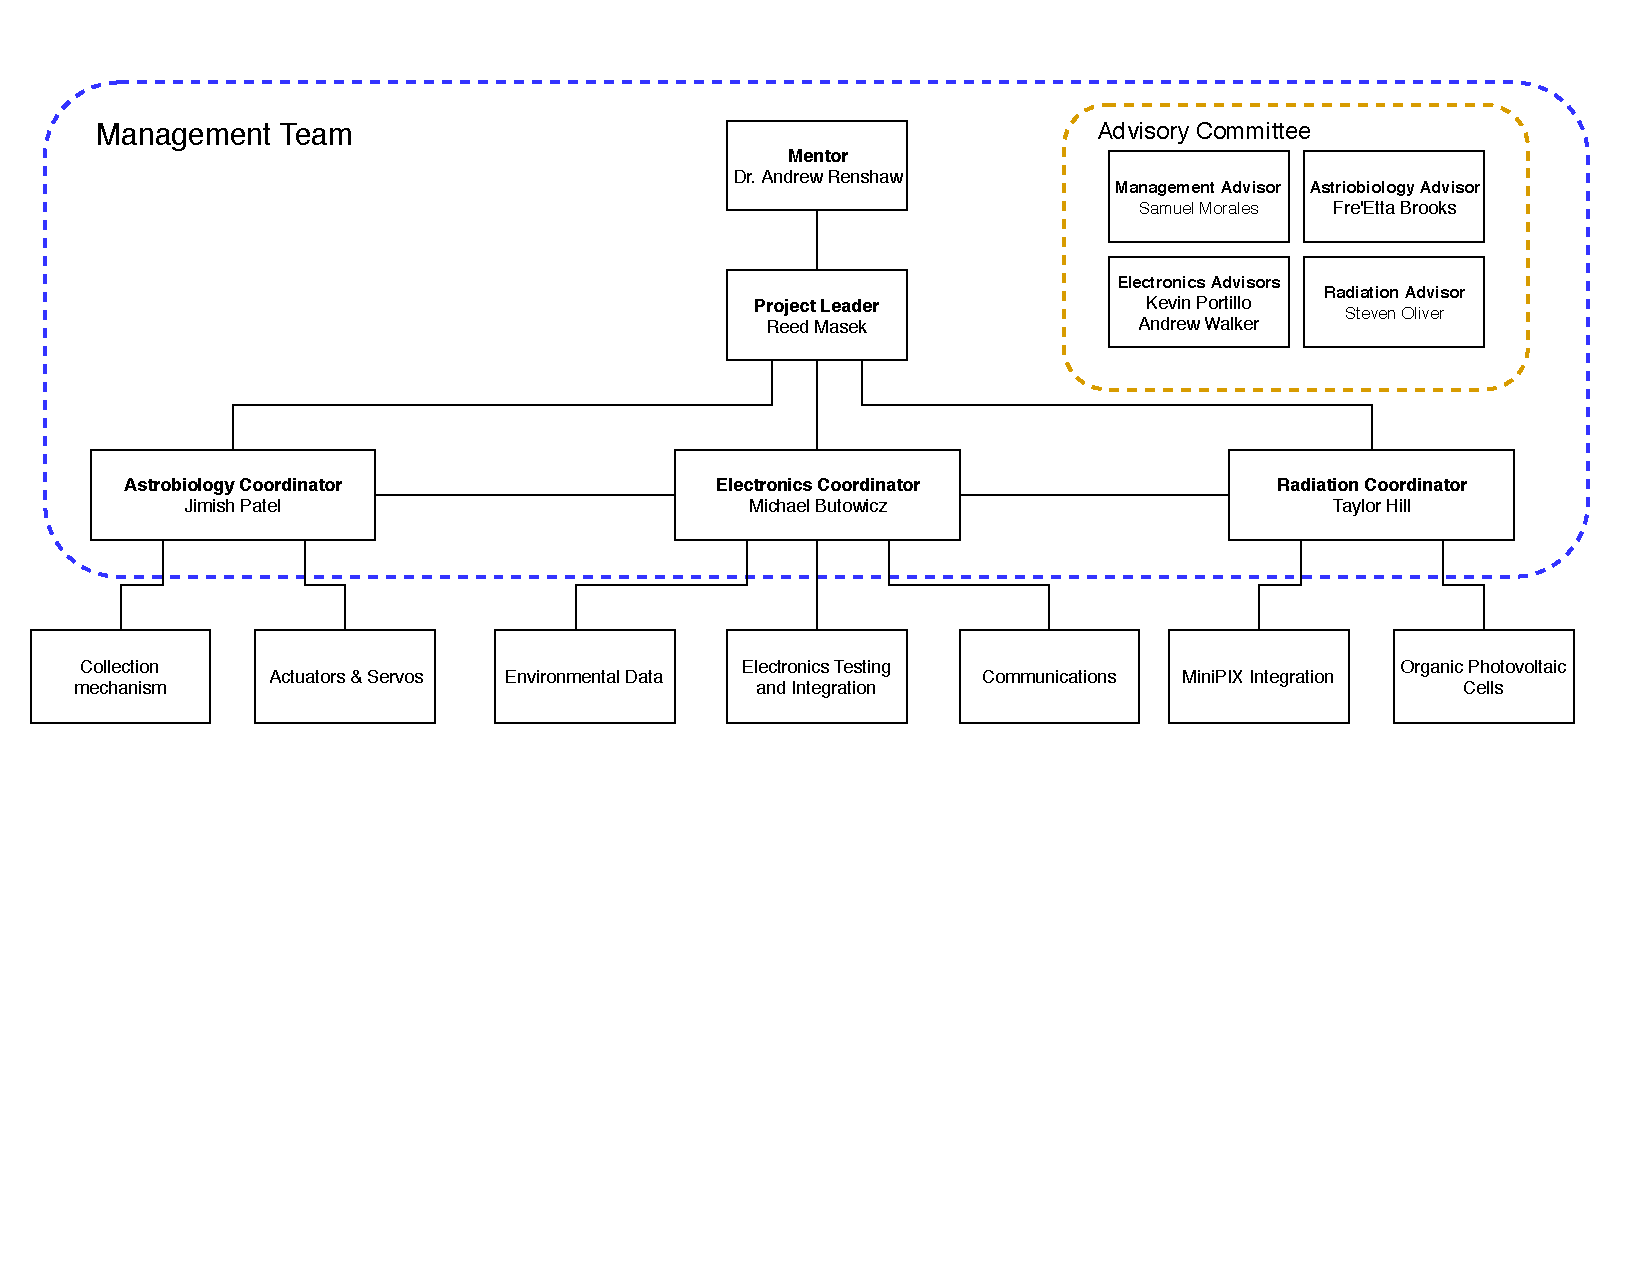
\includegraphics[width=1\textwidth]{./Figures/TeamRoleTree.pdf}
    \caption{Team role tree for the current SORA 2.0 UH team.}
    \label{fig:Roles} 
  \end{center}
\end{figure}

\subsection{Roles and Responsibilities}
\label{sec:Roles}
\begin{itemize}
\item PI – Dr. Andrew Renshaw
	\begin{itemize}
	\item Attend weekly team meetings and provide general research team guidance
	\item Review project design and final products for submission to HASP
	\item Attend monthly teleconferences.
	\item Equipment procurement
	\end{itemize}
\item Project Leader - Reed Masek
	\begin{itemize}
	\item Interface with HASP Flight Control Team and act as team main point of contact
	\item Compile monthly reports and submit to HASP
	\item Attend monthly teleconference with HASP
	\item Coordinate with PI on administration tasks and internal group business
        \item Periodically check-in with team coordinators regarding the team's progress
        \item Coordinate meetings and assign tasks with deadlines
	\item Approve designs, tests, ideas, and any work related to HASP and payload
	\item Final decisions on staffing (staffing decisions will be a group decision overall)
	\end{itemize}
\item Electronics and Communications Coordinator - Michael Butowicz
	\begin{itemize}
	\item Do necessary reserach for finalizing work
	\item Coordinate information, tasks, and deadlines with subgroup
	\item Approve work done by subsystem team
	\item Write bimonthly updates along with detailed reports from subsytem meetings
	\item Make detailed presentations, if necessary, for weekly team meetings
	\item Report to project leader and PI with any project changes, issues encountered, and any external communications.
	\item CC PI and Project Leader in all emails for external communications
	\item Perform other such duties as the Project Leader or PI may specify
	\end{itemize}
\item Astrobiology Coordinator - Jimish Patel
	\begin{itemize}
	\item Do necessary reserach for finalizing work
	\item Coordinate information, tasks, and deadlines with subgroup
	\item Approve work done by subsystem team
	\item Write bimonthly updates along with detailed reports from subsytem meetings
	\item Make detailed presentations, if necessary, for weekly team meetings
	\item Report to project leader and PI with any project changes, issues encountered, and any external communications.
	\item CC PI and Project Leader in all emails for external communications
	\item Perform other such duties as the Project Leader or PI may specify
	\end{itemize}
\item Radiation Coordinator - Taylor Hill
	\begin{itemize}
	\item Do necessary reserach for finalizing work
	\item Coordinate information, tasks, and deadlines with subgroup
	\item Approve work done by subsystem team
	\item Write bimonthly updates along with detailed reports from subsytem meetings
	\item Make detailed presentations, if necessary, for weekly team meetings
	\item Report to project leader and PI with any project changes, issues encountered, and any external communications.
	\item CC PI and Project Leader in all emails for external communications
	\item Perform other such duties as the Project Leader or PI may specify
	\end{itemize}
\item Team Member
	\begin{itemize}
	\item Do necessary reserach for finalizing work
	\item Coordinate with team and subsystem coordinator
	\item Make detailed presentations, if necessary, for weekly team meetings
	\item Report to project leader and PI with any project changes, issues encountered, and any external communications.
	\item CC PI and Project Leader in all emails for external communications
	\item Perform other such duties as the Project Leader or PI may specify
	\end{itemize}
\end{itemize}


\subsection{Timeline}
\label{sec:Timeline}
\begin{table}[H]
\centering
\caption{Timeline for the 2018 SORA 2.0 Mission}
\label{timeline}
\resizebox{\textwidth}{!}{%
\begin{tabular}{|c|l|}
\hline
\textbf{Month of 2018} & \multicolumn{1}{c|}{\textbf{Description of Work}} \\ \hline
\textbf{January} & \begin{tabular}[c]{@{}l@{}} * Secure funding \\ * Create and finish budget for mission \\ * Make inventory of hardware \\ * Procure hardware/software \\ * Start designs of SORA 2.0 \\ * Update RESU \\ * Upgrade vacuum chamber \\ * Recruit new members \end{tabular} \\ \hline
\textbf{February} & \begin{tabular}[c]{@{}l@{}}
* Continue with work from January.  Funding must be secured by end of March.\\ * Have finished list of inventory\\ * Finalize upgrades to vacuum chamber\\ * Continue recruitment and finalize by end of month.\\ * Continue design work of SORA 2.0\\ * Finish RESU upgrade\end{tabular} \\ \hline
\textbf{March} & \begin{tabular}[c]{@{}l@{}}Obtain funding by the end of this month.  Finish all tasks from the previous two months and transition into building phase.\\ * Have all hardware/software orders in by the end of the month\\ * Begin PSIP, have draft by end of the month\end{tabular} \\ \hline
\textbf{April} & \begin{tabular}[c]{@{}l@{}}* Order remaining items if needed\\ * Finish PSIP by April 25th\\ * RESU and MiniPIX integration and testing\\ * Upgrade clean room and prepare for astrobiology work\end{tabular} \\ \hline
\textbf{May} & \begin{tabular}[c]{@{}l@{}}* PSIP and FLOP development\\ * Finalize integration of RESU and hardware\\ * Continue working on astrobiology upgrades\end{tabular} \\ \hline
\textbf{June} & \begin{tabular}[c]{@{}l@{}}Final PSIP due June 27th\\ *Finalize astrobiology upgrades and ready for integration\\ * Testing in lab\end{tabular} \\ \hline
\textbf{July} & \begin{tabular}[c]{@{}l@{}}Final FLOP due July 31st\\ * Make changes from testing and continue tests\end{tabular} \\ \hline
\textbf{August} & \begin{tabular}[c]{@{}l@{}}Payload Integration (August 4 - 8)\\ *Have all payload work done and ready for flight\end{tabular} \\ \hline
\textbf{September} & * Launch and recovery TBA \\ \hline
\textbf{October} & Debrief and analyze all data from flight \\ \hline
\textbf{November} & Have final report by end of November \\ \hline
\textbf{December} & Final Report due on the 8th \\ \hline
\end{tabular}%
}
\end{table}


\subsection{Funding}
\label{sec:Funding}


%Funding sources will be local contributions - applying for funding through the Physics Department, the College of Natural Science and Mathematics, The University of Houston Division of Research, and local organizations and companies willing to support this endeavor.  


\newpage
\section{Appendix A}
\label{sec:Appendix A}

\subsection{Payload Dimensions}

	
\newpage

\begin{thebibliography}{9}
\bibitem{SORA1}
S.A. Garcia Morelos, F. Brooks, S. Oliver, A. Walker, K.D. Portillo, R.B. Masek, D. Mroczek, D. Pena, J. Juarez, A. Cruz, D. Henandez, S. George, D. Pattison, A.L. Renshaw. \textit{Scientific Report for the 2017 UH Team.} SORA 2017 Mission Webpage. \url{http://laspace.lsu.edu/hasp/groups/Payload.php?py=2017&pn=10}.

\bibitem{SORA2}
  S. A. Garcia Morelos, F. Brooks, S. Oliver, A. Walker, K. D. Portillo, R. B. Masek, J. Patel, S. George, I. Wilson, D. Pattison, P. Gunaratne, and A. L. Renshaw. \textit{SORA 2.0: Stratospheric Organism and Radiation Analyzer}

\bibitem{MiniPIX}
  MiniPIX - Miniaturized Portable USB Photon Counting Camera. (n.d.). Retrieved February 02, 2017, from \url{http://advacam.com/camera/minipix}.

\bibitem{Regener}
 Regener E. \& Pfotzer G., \textit{Vertical Intensity of Cosmic Rays by Threefold Coincidences in the Stratosphere.}, Nature 136, 718-719, (1935). 
  
\bibitem{LSU}
  Christner, B., Alleman, M., Bryan, N., Burke, S., Guzik, T.G., Granger, D., King, G. (2013) \textit{LSU HASP2013 PDF. Baton Rouge: Louisiana Space Consortium}.

\bibitem{Extremophiles}
  Extremophiles \href{http://www.nytimes.com/2013/02/07/science/living-bacteria-found-deep-under-antarctic-ice-scientists-say.html}{http://www.nytimes.com/2013/02/07/science/living-bacteria-found-deep-\\under-antarctic-ice-scientists-say.html}.

\bibitem{Frank}
  Schröder, F. G. (2017). Radio detection of cosmic-ray air showers and high-energy neutrinos. Progress in Particle and Nuclear Physics, 93, 1-68. doi:10.1016/j.ppnp.2016.12.002

\bibitem{GCRs}
  https://helios.gsfc.nasa.gov/gcr.html

\bibitem{Hathaway}
  Hathaway, D. H. (2015). The Solar Cycle. Living Reviews, 12. doi:10.1007/lrsp-2015-4
  
\bibitem{NASA HRP}
  https://www.nasa.gov/hrp

\bibitem{NASAShielding}
  National Research Council. 1997. \textit{Protecting the Space Station from Meteoroids and Orbital Debris}. Washington, DC: The National Academies Press. \url{https://doi.org/10.17226/5532}.

\bibitem{NASAPP}
  Christiansen, E. L., Lear, D. M. (2012). Micrometeoroid and Orbital Debris Environment \& Hypervelocity Shields [PowerPoint slides]. Retrieved from \url{https://ntrs.nasa.gov/archive/nasa/casi.ntrs.nasa.gov/20120002584.pdf}.
  
\bibitem{SolarEnergyMaterials}
  Solar Energy Materials and Solar Cells 182 (2018) 121–127 DOI: 10.1016/j.solmat.2018.03.024.

\bibitem{Kaltenbrunner}
  Kaltenbrunner, M. et al. Ultrathin and lightweight organic solar cells with high flexibility. Nat. Commun. 3:770 DOI: 10.1038/ncomms1772 (2012).

\bibitem{Uher}
  Uher, J., Frojdh, C., Holy, T., Jakubek, J., Petersson, S., Pospisif, S., . . . Stekl, I. (2007). Silicon Detectors for Neutron Imaging. AIP Conference Proceedings. doi:10.1063/1.2825756

\bibitem{BoronScintillator}
  EJ-254 Boron Loaded Plastic Scintillator \url{https://eljentechnology.com/images/products/data_sheets/EJ-254.pdf}.

\bibitem{Pawelczak}
  Pawełczak, I., Glenn, A., Martinez, H., Carman, M., Zaitseva, N., \& Payne, S. (2014). Boron-loaded plastic scintillator with neutron-$\gamma$ pulse shape discrimination capability. Nuclear Instruments and Methods in Physics Research Section A: Accelerators, Spectrometers, Detectors and Associated Equipment, 751, 62-69. doi:10.1016/j.nima.2014.03.027
  
\bibitem{Canales}
 Canales D. C. and Ehteshami A., \textit{An attempt to sample atmospheric bacteria}, Houston, TX, 2015, January 11.

\bibitem{Bexus}
Urbar, J., Scheirich, J., Jakubek, J., 2011. Medipix/Timepix cosmic ray tracking on BEXUS stratospheric balloonflights. Nucl. Instrum. Methods A 633, S206-209.

\bibitem{Advacam}
  ADVACAM at \url{advacam.com}.

\bibitem{Medipix}
  Medipix collaboration at \url{https://medipix.web.cern.ch/}.
  
\bibitem{StuartThesis} 22
  George, S., \textit{Dosimetric Applications of Hybrid Pixel Detectors}, University of Wollongong, Australia, 2015.
  
  \bibitem{OPV_operation}
  DOI: 10.1038/nmat3807 
  
  \bibitem{OSCAR}
  Solar Energy Materials and Solar Cells 182 (2018) 121–127
DOI: 10.1016/j.solmat.2018.03.024

\bibitem{NASAorganics}
\url{https://ntrs.nasa.gov/search.jsp?R=20030016569}

\bibitem{Space organic cells}
Sheila Bailey and Ryne Raffaelle, Space Solar Cells and Arrays

\bibitem{nextgen_TCO}
Kuan Sun, Yijie Xia, and Jianyong Ouyang, Next-Generation transparent electrode materials for organic solar cells


%\bibitem{uv_irradiance}
%  Calculating the UV Index. (2016, October 14). Retrieved June 03, 2017, from \url{https://www.epa.gov/sunsafety/calculating-uv-index-0}.

%\bibitem{cleanbox}
% Clean box material \url{https://www.mcmaster.com/\#uhmw-polyethylene/=1aijn1p}.

%\bibitem{Valve}
 %Valve data sheet \url{http://www.generant.com/Literature/Series\%20VRV\%20Product\%20Literature.pdf}.

%\bibitem{mpdatasheet}
%  ADVACAM, \textit{MINIPIX Version 1.0 Datasheet}, Retrieved from \url{http://www.widepix.cz/files/datasheets/MiniPIX\%20v1.0\%20Datasheet.pdf}.

%\bibitem{mpjakubek}
%  Jan Jakubek, \textit{Precise energy calibration of pixel detector working in time-over-threshold mode} Institute of Experimental and Applied Physics, Czech Technical University in Prague, Czech Republic, 2011.
  
%\bibitem{magnetictool}
%  United States National Oceanic and Atmospheric Administration, \textit{Magnetic Field Calculators} [Data sets], Retrieved from \url{https://www.ngdc.noaa.gov/geomag-web/#igrfwmm}.

%\bibitem{gorman}
%	Gorman, J. (2013, February 06). \textit{Scientists Find Life in the Cold and Dark Under Antarctic Ice.} Retrieved September 15, 2016, from Scientists Find Life in the Cold and Dark Under Antarctic Ice.
 
%\bibitem{pumpsource}
%  \url{http://www.knfusa.com/?type=5600&amp;file=2079}.

%\bibitem{Horneck}
%  Horneck, G. 1993. The Biostack concept and its application in space and at accelerators: studies in Bacillus subtilis spores, p. 99-115. In C. E. Swenberg, G. Horneck, and E. G. Stassinopoulos (ed.), \textit{Biological effects and physics of solar and galactic cosmic radiation}[PDF], part A. Plenum Press, New York, NY. accessed 10/24/16  

%\bibitem{Horneck} 
%  Horneck, G. 2007. \textit{Space radiation biology}[PDF], p. 243-273. In E. Brinckmann (ed.), Biology in space and life on Earth. Wiley-VCH, Weinheim, Germany. Accessed 10/26/16

%\bibitem{Horneck}
%  Horneck, G., C. Baumstark-Khan, and G. Reitz. 2002. \textit{ Space microbiology: effects of ionizing radiation on microorganisms in space}[PDF], p. 2988-2996. In G. Bitton (ed.), The encyclopedia of environmental microbiology. John Wiley \& Sons, New York, NY. Accessed 10/30/16

%\bibitem{Horneck}
%  Horneck, G., C. Baumstark-Khan, and R. Facius. 2006. \textit{Radiation biology}[PDF], p. 292-335. In G. Cl?ment and K. Slenzka (ed.), Fundamentals of space biology. Kluwer Academic Publishers/Springer, Dordrecht, The Netherlands. accessed 11/4/16

%\bibitem{Kiefer}
%Kiefer, J., K. Schenk-Meuser, and M. Kost. 1996. \textit{Radiation biology}[PDF], p. 300-367. In D. Moore, P. Bie, and H. Oser (ed.), Biological and medical research in space. Springer, Berlin, Germany. accessed 11/9/16

%\bibitem{SamURD}
 % Alfonso Garcia Morelos, S. (2016, October 13).
 % \textit{A Novel Microbe Trap.}
 % Presentation at UH Undergraduate Research Day. \url{http://www.uh.edu/honors/undergraduate-research/}
  
%\bibitem{SamAPS}
%	Alfonso Garcia Morelos, S. (2017, October 20).
%	\textit{Stratospheric Organism and Radiation Analyzer}
%	Retrieved October 20, 2017, from \textit{Bulletin of the American Physical Society}. \url{https://meetings.aps.org/Meeting/TSF17/Session/E5.3}
	
%\bibitem{StevenURD}
%  Oliver, S. J. (2017, October 12). 
%  \textit{Stratospheric Organism and Radiation Analyzer}
%  Presentation at UH Undergraduate Research Day. Retrieved October 12, 2017, from \url{http://www.uh.edu/honors/undergraduate-research/events/urday2017/}

%\bibitem{StevenSchoolPres}
%  Oliver, S. J. (2017, November 4). 
%  \textit{STEM Life at UH}
%  Presentation at UH Gathering of the Eagles STEM Symposium. \url{https://www.uh.edu/news-events/stories/2016/November/110416EaglesSTEM.php}

%\bibitem{Fre}
%  Brooks, F. (2017, January 14).
%  \textit{Stratospheric Organism and Radiation Analyzer}
%  Presentation at Rice University, APS Conferences for Undergraduate Women in Physics (CUiP). \url{http://www.google.com/url?q=http%3A%2F%2Fwww.aps.org%2Fprograms%2Fwomen%2Fworkshops%2Fcuwip.cfm&sa=D&sntz=1&usg=AFQjCNE5pImV-SVrb87CvgAa9RSfeCrYXg}  
  
\end{thebibliography}



\end{document}
